\documentclass{beamer}
\usepackage[utf8]{inputenc}
%\usepackage{0_slides}
\usepackage[russian]{babel}
\usepackage{amsmath,mathrsfs,mathtext}
\usepackage{graphics,graphicx,epsfig}
\usepackage{epstopdf}
\usepackage{fancybox,fancyhdr}
\usepackage{enumerate}
\usepackage{array}
\usepackage[version=0.96]{pgf}
\usepackage{tikz}
\usepackage[normalem]{ulem}
\usepackage{arydshln}
\usepackage{multicol, multirow}


\usepackage{../NotationStyle}

\setlength\dashlinedash{0.2pt}
\setlength\dashlinegap{4.5pt}


\usetheme{default} \usecolortheme{whale}
\setbeamertemplate{blocks}[rounded=false, shadow=false]

\definecolor{beamer@blendedblue}{RGB}{15,120,80}
\renewcommand{\thefootnote}{\fnsymbol{footnote}}

\newcommand\Wider[2][3em]{%
\makebox[\linewidth][c]{%
  \begin{minipage}{\dimexpr\textwidth+#1\relax}
  \raggedright#2
  \end{minipage}%
  }%
}
\newcommand{\argmax}{\mathop{\rm arg\,max}\limits}

\graphicspath{ {../../code/} {../fig/} {fig/}}

%-----------------------------------------------------------------------------------------------------
\title[\hbox to 56mm{Multiscale forecasting\hfill\insertframenumber\,/\,\inserttotalframenumber}]{Feature generation for multiscale time series forecasting}
\author[V. Strijov]{A. Motrenko, R. Neychev, R. Isachenko, M. Popova, V. Strijov}
\institute{Moscow Institute of Physics and Technology}
\date{2016}

%-----------------------------------------------------------------------------------------------------
\begin{document}
\begin{frame}
\maketitle
\end{frame}
%==================================================================================================
\begin{frame}{Outline}


\begin{itemize}
\item Design matrix
\item Testing procedure
\item Feature generation
\item Feature selection
\item Mixture models
\item Resampling
\end{itemize}

\end{frame}
%-----------------------------------------------------------------------------------------------------
\begin{frame}
\vfill
\begin{center}
{\Large \bf Problem statement}
\end{center}
\vfill
\end{frame}
%-----------------------------------------------------------------------------------------------------
%------------------------------------------------------------------------------------------------------
\begin{frame}{Energy consumption one-week forecast for each hour}%, hierarchical algorithms}

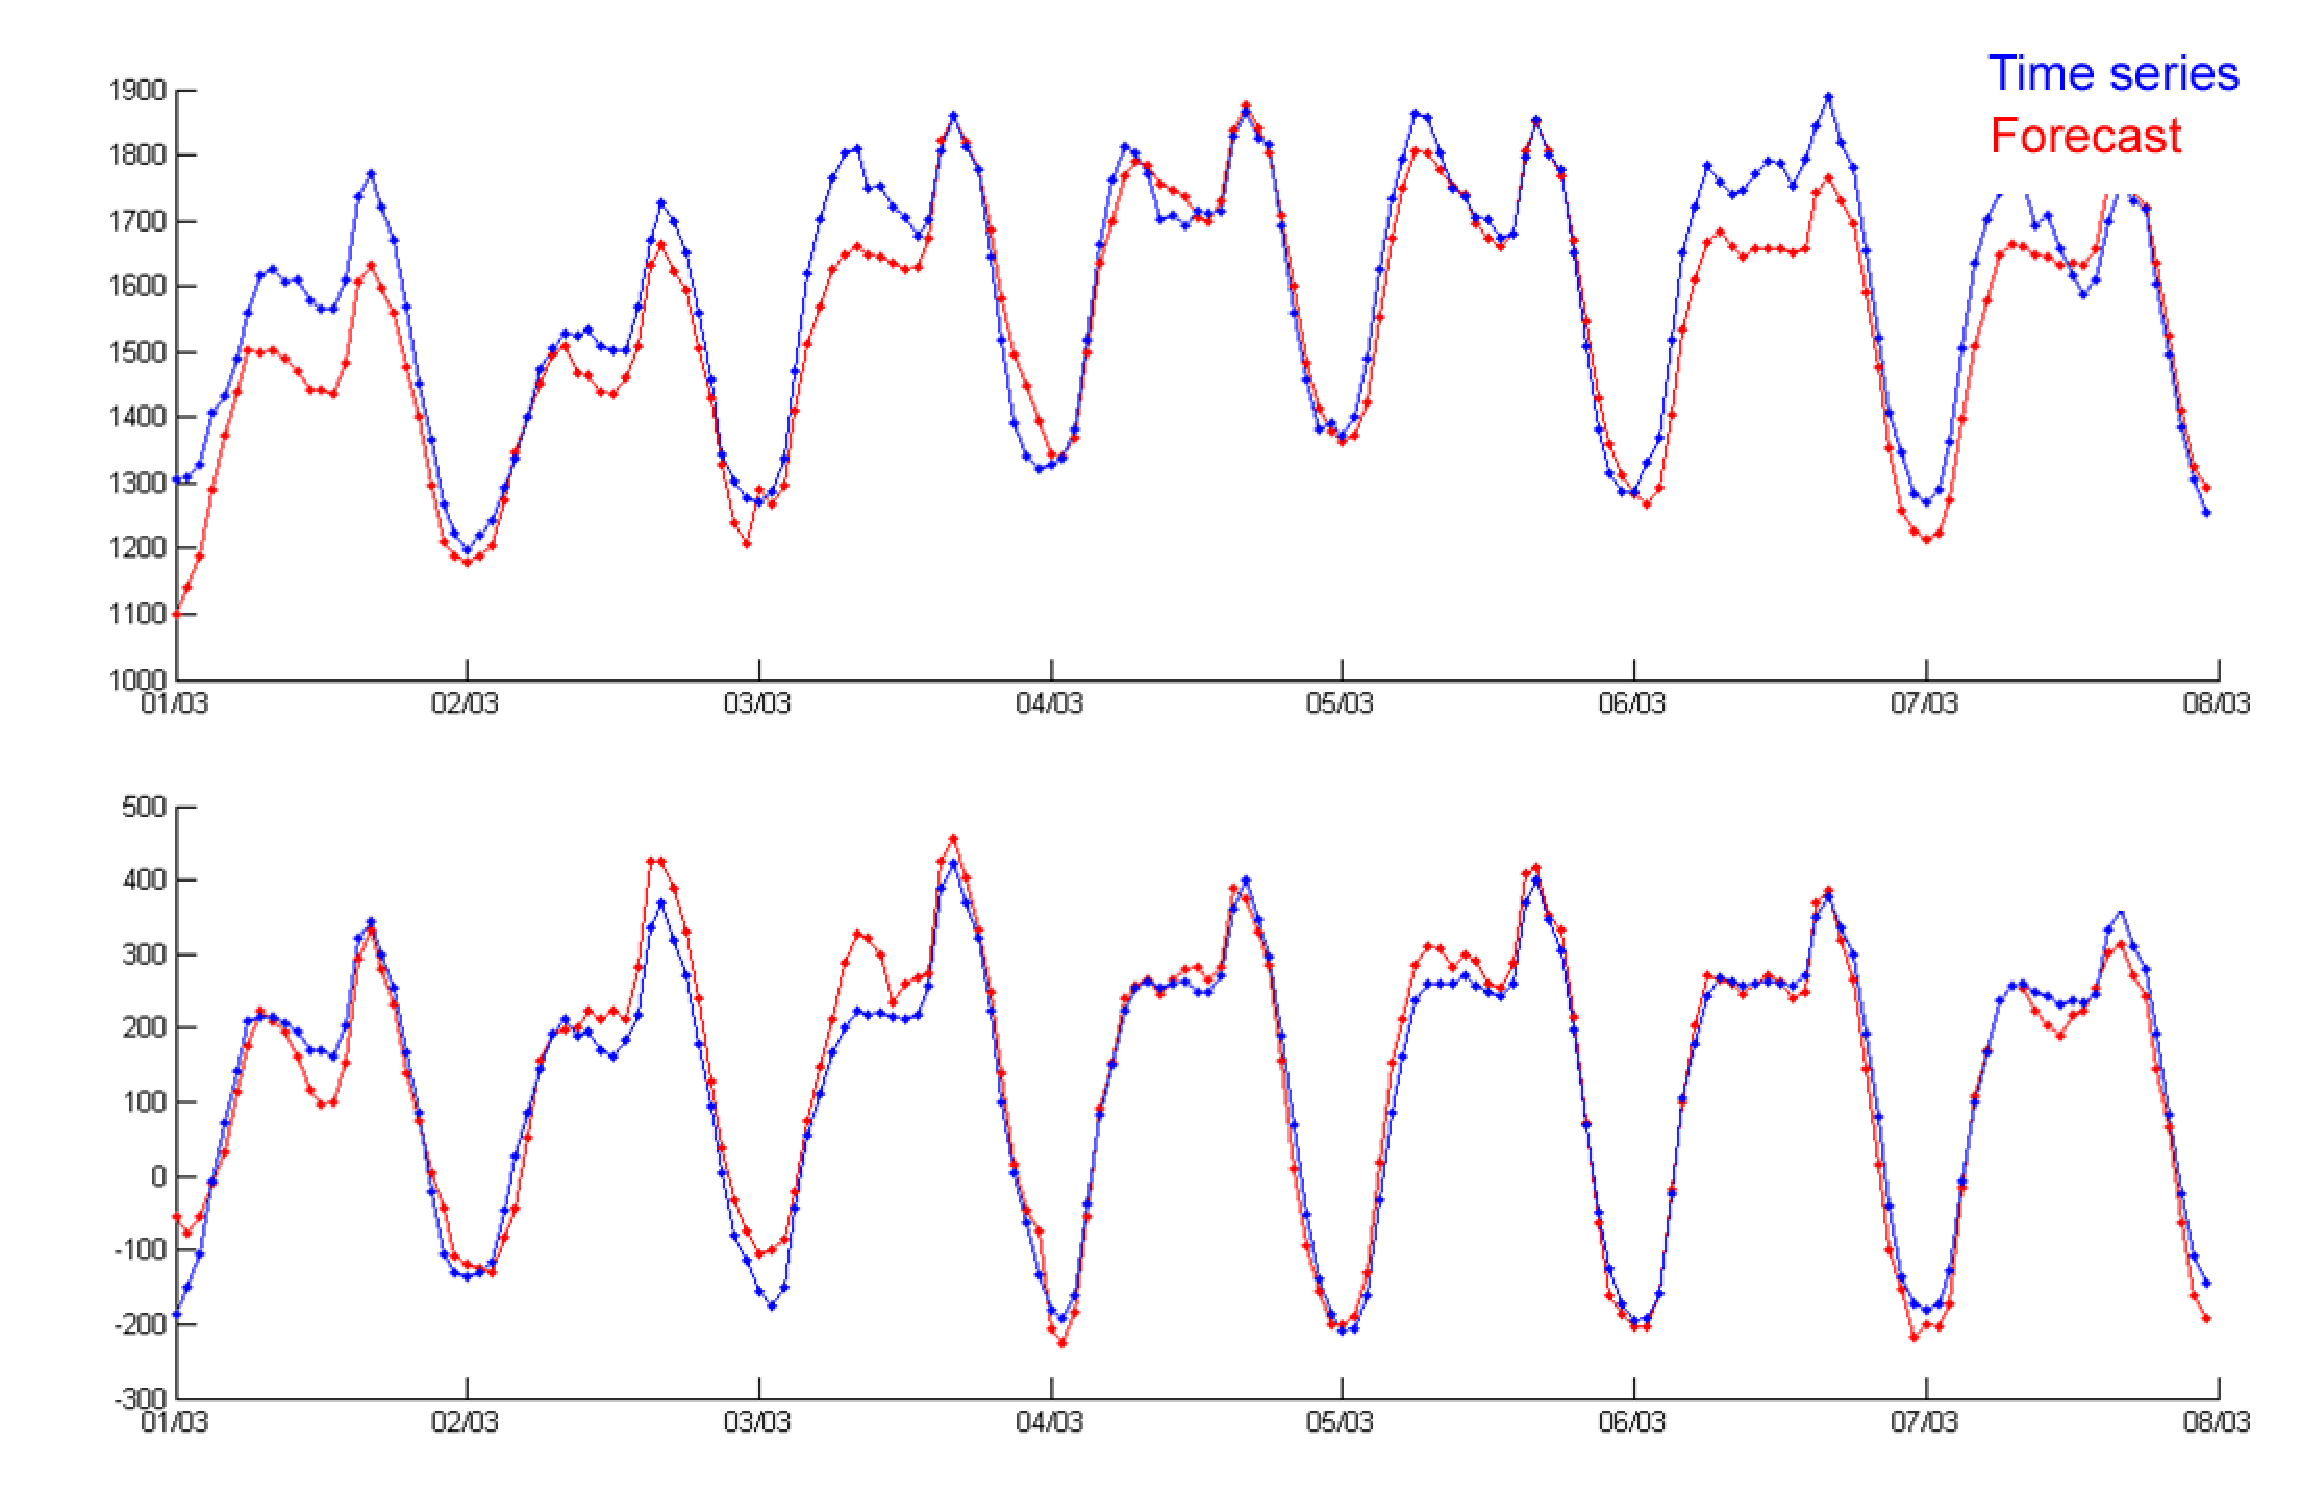
\includegraphics[width=\textwidth]{fig/fig9.eps}
\end{frame}

\begin{frame}[t]{The periodic components of the multivariate time series}

\vfill
\begin{columns}[c]
\column{1.5in}
   The time series:

   \bigskip
   \begin{itemize}
       \item energy price,
       \item consumption,
       \item daytime,
       \item temperature,
       \item humidity,
       \item wind force,
       \item holiday schedule.
   \end{itemize}
\column{1.5in}
   Periods:

   \bigskip
   \begin{itemize}
       \item one year seasons (temperature, daytime),
       \item one week,
       \item one day (working day, week-end),
       \item a holiday,
       \item aperiodic events.
   \end{itemize}

\column{1.5in}
   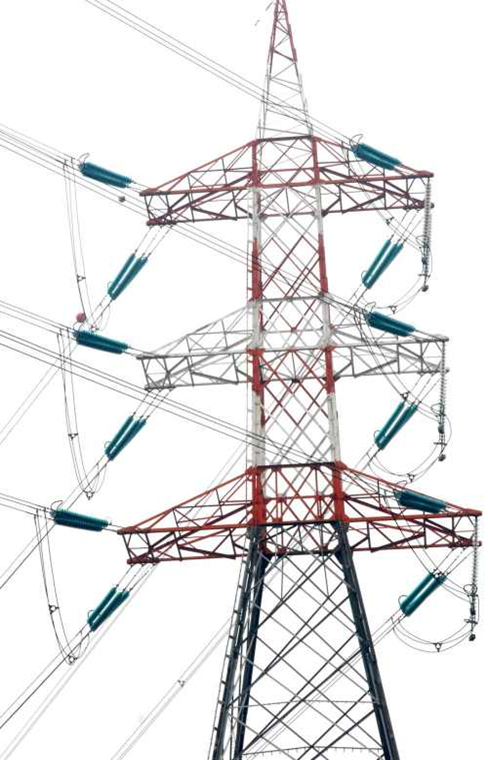
\includegraphics[width=2in]{fig/fig0.png}
\end{columns}
\vfill
\end{frame}
%-----------------------------------------------------------------------------------------------------
\begin{frame}[t]{The autoregressive matrix, five week-ends}

\begin{center}
{\includegraphics[width=0.75\textwidth]{fig/Weeks5.eps}}
\end{center}

\end{frame}
%-----------------------------------------------------------------------------------------------------
\begin{frame}{The autoregressive matrix and the linear model}
$$
\underset{(m+1)\times(n+1)}{\mathbf{X}^*}  =
\left(%
\begin{array}{l|lll}
s_T                 & s_{T-1}           & \ldots & s_{T-\kappa +1}      \\
\hline                                                                  \\
s_{(m-1)\kappa }    & s_{(m-1)\kappa -1}& \ldots & s_{(m-2)\kappa +1}   \\
\ldots              & \ldots            & \ldots & \ldots               \\
s_{n\kappa }        & s_{n\kappa -1}    & \ldots & s_{n(\kappa -1)+1}   \\
\ldots              & \ldots            & \ldots & \ldots               \\
s_\kappa            & s_{\kappa -1}     & \ldots & s_1                  \\
\end{array}%
\right).
$$

\bigskip
In a nutshell,
$$
\mathbf{X}^*=\left[
\begin{array}{c|c}
 \underset{1{\times}1}{s_T} & \underset{1{\times}n}{\x_{m+1}} \\
 \hline
 \underset{m{\times}1}{\mathbf{y}} & \underset{m{\times}n}{\mathbf{X}} \\
\end{array}
\right].
$$

In terms of linear regression:
$$
\mathbf{y} = \mathbf{X}\mathbf{w},
$$
$$
y_{m+1} = s_T = \w\T\x_{m+1}\T.
$$
\end{frame}
%-----------------------------------------------------------------------------------------------------
\begin{frame}{Model generation}
%
Introduce a set of the primitive functions $\mathfrak{G}=\{g_1,\ldots,g_r\}$, \par
for example $g_1=1$, $g_2=\sqrt{x}$, $g_3=x$, $g_4=x\sqrt{x}$, etc.

\vspace{0.7cm}
The generated set of features $\mathbf{X}=$
{\footnotesize
$$
\left(%
\begin{array}{lll|l|lll}%
g_1\circ s_{T-1}    & \ldots & g_r\circ s_{T-1}        & \ldots & g_1\circ s_{T-\kappa +1} & \ldots   & g_r\circ s_{T-\kappa +1}\\
\hline
g_1\circ s_{(m-1)\kappa -1}& \ldots & g_r\circ s_{(m-1)\kappa -1}   & \ldots & g_1\circ s_{(m-2)\kappa +1} & \ldots & g_r\circ s_{(m-2)\kappa +1} \\
\ldots      & \ldots & \ldots        & \ldots & \ldots  & \ldots      & \ldots\\
g_1\circ s_{n\kappa -1}    & \ldots & g_r\circ s_{n\kappa -1}       & \ldots & g_1\circ s_{n(\kappa -1)+1} & \ldots & g_r\circ s_{n(\kappa -1)+1}\\
\ldots      & \ldots & \ldots        & \ldots & \ldots  & \ldots      & \ldots\\
g_1\circ s_{\kappa -1}     & \ldots & g_r\circ s_{\kappa -1}        & \ldots & g_1\circ s_1  & \ldots         & g_r\circ s_1\\
\end{array}%
\right).
$$
}

Kolmogorov-Gabor polynomial as a variant for model generation
$$
y=w_0+\sum_{i=1}^{UV}w_ix_i + \sum_{i=1}^{n}\sum_{j=1}^{n}w_{ij}x_ix_j +\dots + \sum_{i=1}^{n}\ldots\sum_{z=1}^{n}w_{i\ldots z}x_i\ldots x_z,
$$
where the coefficients
$$
\mathbf{w}= (w_0,w_i,w_{ij},\ldots,w_{i\ldots z})_{i,j,\ldots,z=1,\ldots,n}.
$$

\end{frame}
%-----------------------------------------------------------------------------------------------------
\begin{frame}[t]{The one-day forecast (an example)}

{\hfill\includegraphics[angle=0,width=0.75\textwidth]{fig/Forecast1.eps}\hfill}

The function $y  =  f(\mathbf{x}, \mathbf{w})$ could be a linear model, neural network, deep NN, SVN, ...

\end{frame}
%-----------------------------------------------------------------------------------------------------
\begin{frame}{Ill-conditioned matrix, or curse of dimensionality}

Assume we have hourly data on price/consumption for three years.

Then the matrix~$\underset{(m+1)\times(n+1)}{\mathbf{X}^*}$  is
\begin{center}
$156 \times 168$, in details: $52\mbox{w} \cdot 3\mbox{y} \times 24\mbox{h}\cdot 7\mbox{d}$;
\end{center}

\begin{itemize}
\item for 6 time series the matrix $\mathbf{X}$ is $156 \times 1008$,
\item for 4 primitive functions it is $156 \times 4032$,
\end{itemize}
$$
m<<n.
$$

The autoregressive matrix could be considered as \emph{ill-conditioned} and \emph{multi-correlated}.
The model selection procedure is required.
\end{frame}
%-----------------------------------------------------------------------------------------------------
\begin{frame}[t]{How many parameters must be used to forecast?}
The color shows the value of a parameter for each hour.

{\hfill{\includegraphics[angle=0,width=0.6\textwidth]{fig/FlatParameters.eps}}\hfill}

Estimate parameters~$\mathbf{w}(\tau)=(\mathbf{X}\T \mathbf{X})^{-1}\mathbf{X}\T\mathbf{y}$,
then calculate the sample $s(\tau) = \w\T (\tau) \mathbf{x}_{m+1}$ for each~$\tau$ of the next ($m+1$-th) period.
%
%\begin{itemize}
%\item $\mathbf{w}=(X^TX)^{-1}X^T\mathbf{y}$
%\item $s(T) = \langle{\mathbf{x}_m, w}\rangle$
%\item for each~$j$ of the next period.
%\end{itemize}
\end{frame}
%-----------------------------------------------------------------------------------------------------
\begin{frame}[t]{Ways to model selection: brief list of algorithms}
Exhaustive search and modifications
\begin{enumerate}
\item Exhaustive search of $2^P$ models
%\item Method of group data handling, $K \cdot C_P^2$ models
\item Genetic algorithms
\item Add/Del (append/delete a feature), $P(P-1)/2$ models
\item Add-del or stepwise regression, $\sim P^2$ models
\end{enumerate}

\vspace{0.7cm}
Parameter space analysis
\begin{enumerate}
\item Least angle regression, Lasso, Stagewise, Elastic net
\item Optimal brain damage/surgery
\end{enumerate}
\end{frame}
%-----------------------------------------------------------------------------------------------------
\begin{frame}[t]{Exhaustive search and Add algorithms}
\vspace{-.5cm}
The initial model includes all independent variables
$$
f(\mathbf{w},\mathbf{x}) = \alpha_1 w_1 x_1 + \alpha_2 w_2 x_2 + \ldots +\alpha_n w_n x_n.
$$
The hyperparameter $\alpha\in\{0,1\}$ is included in the model. The {\bf exhaustive search} procedure counts
$$
\begin{array}{cccc}
\alpha_1 & \alpha_2 & \ldots & \alpha_n \\
\hline
1 & 0 & \ldots & 0 \\
0 & 1 & \ldots & 0 \\
\ldots & \ldots & \ldots & \ldots \\
1 & 1 & \ldots & 1 \\
\end{array}.
$$
%\end{frame}
%%-----------------------------------------------------------------------------------------------------
%\begin{frame}[t]

{\bf Add (append a feature)}

\begin{enumerate}
\item[Step~0.]
The active set $\mathcal{A}_0=\emptyset$.
\item[Step~~$k$]$=1,\ldots,n$.
Select the next best feature index
$$
\hat{j}=\arg\min_{j\in \{1,\dots,n\}\setminus\mathcal{A}_k}\text{~}\min\limits_{\mathbf{w}\in\mathbb{R}^{|\mathcal{A}|}}\|[\mathbf{X}_{\mathcal{A}_{k}}\boldsymbol{\chi}_j]\mathbf{w}-\mathbf{y}\|_2^2,
$$
according to minimum of the error function $S(\mathbf{w})$; then
$$
\mathcal{A}_{k+1}=\mathcal{A}_k\cup\hat{j}.
$$
\end{enumerate}
\end{frame}

%-----------------------------------------------------------------------------------------------------
\begin{frame}[t]{Discrete genetic algorithm for feature selection (simple ver.)}
\vfill
\begin{enumerate}
\item There are set of binary vectors $\{\mathbf{a}_1,\ldots,\mathbf{a}_P\}$, $\mathbf{a}\in\{0,1\}^n$;
\item get two vectors $\mathbf{a}_p, \mathbf{a}_q$, $p,q\in\{1,\ldots,P\}$;
\item chose random number $\nu\in \{1,\ldots,n-1\}$;
\item split both vectors and change their parts:
$$[a_{p,1},\ldots,a_{p,\nu},a_{q,\nu+1},\ldots,a_{q,n}]\to\mathbf{a'}_p,$$
$$[a_{q,1},\ldots,a_{q,\nu},a_{p,\nu+1},\ldots,a_{p,n}]\to\mathbf{a'}_q;$$
\item choose random numbers $\eta_1,\ldots,\eta_Q\in\{1,\ldots,n\}$;
\item invert positions $\eta_1,\ldots,\eta_Q$ of the vectors $\mathbf{a'}_p,\mathbf{a'}_q$;
\item repeat items 2-6 $P/2$ times;
\item evaluate the obtained models.
\end{enumerate}
\vfill
Repeat $R$~times; here $P,Q,R$ are the parameters of the algorithm and~$n$ is the number of the corresponding model features.
\end{frame}

%----------------------------------------------------------------------------------------------------------
\begin{frame}[c]{Selection of a stable set of features of restricted size}

{\small
The sample contains multicollinear~$\bchi_1, \bchi_2$ and noisy~$\bchi_5,\bchi_6$ features, columns of the design matrix~$\bX$. We want to select two features from six.}

\begin{center}
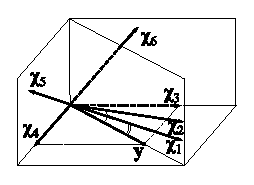
\includegraphics[width=0.5\textwidth]{exp3_1.eps}
\end{center}

\begin{block}{Stability and accuracy for a fixed complexity}
The solution:~$\bchi_3,\bchi_4$is an orthogonal set of features minimizing the error function.
\end{block}

{\tiny Algorithms: GMDH, Stepwise, Ridge, Lasso, Stagewise, FOS, LARS, Genetics, ... }

\end{frame}
%----------------------------------------------------------------------------------------------------------
\begin{frame}{Model parameter values with regularization}
Vector-function~$\fx =\fx(\w,\bX)=[f(\w,\x_1),\ldots,f(\w,\x_m)]\T \in \mathbb{Y}^m$.
\begin{columns}[c]
\column{0.5\textwidth}
\centering 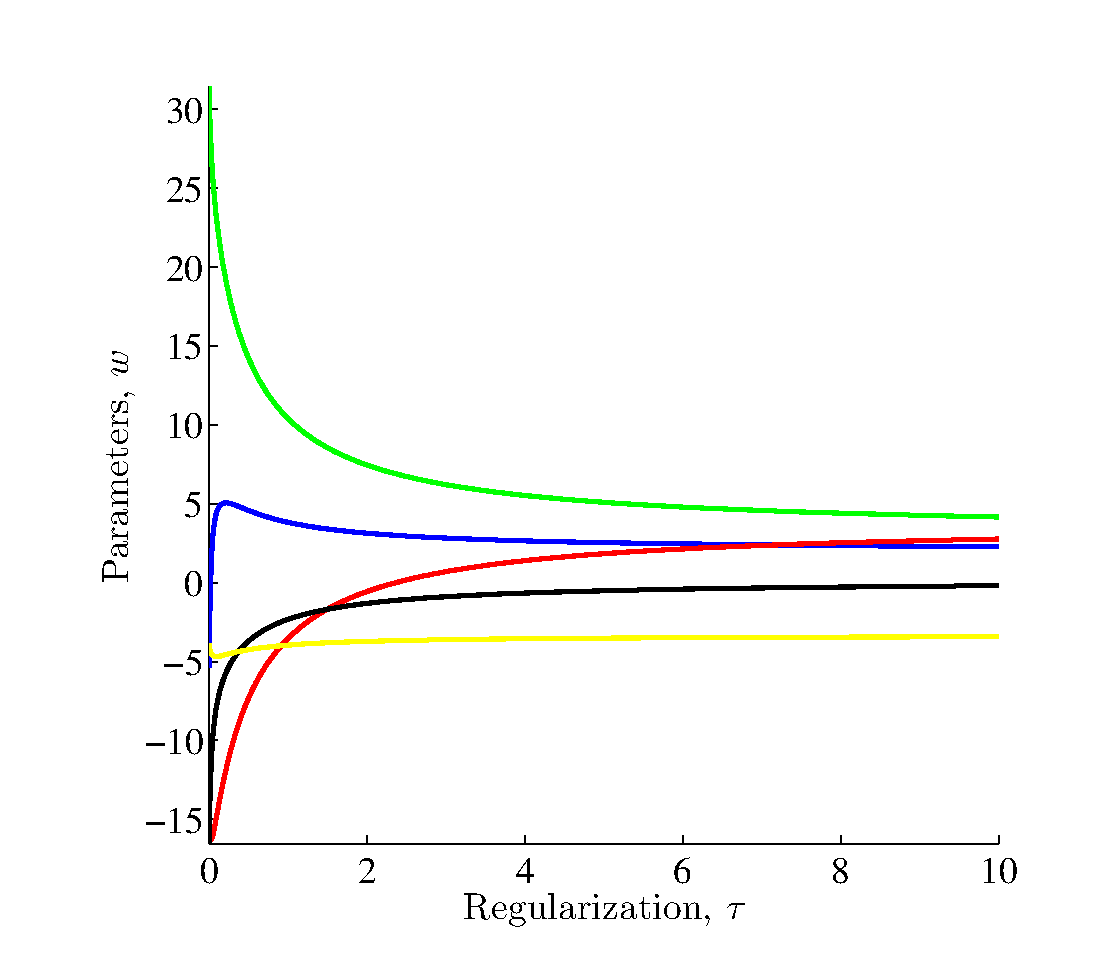
\includegraphics[width=\textwidth]{ridgeparams.eps}  \par $S(\bw)= \|\fx(\bw,
\bX)-\by\|^2 + \gamma^2\|\bw\|^2$
\column{0.5\textwidth}
\begin{center}
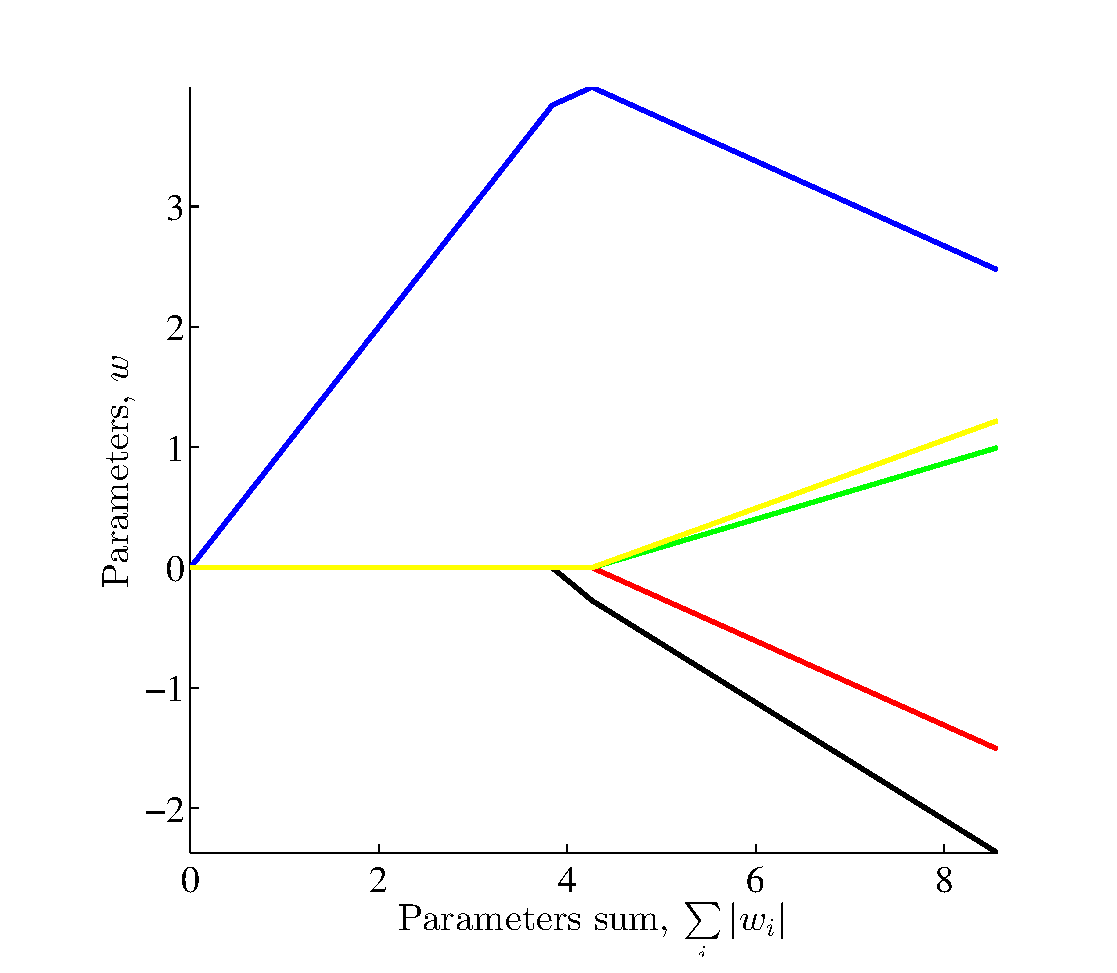
\includegraphics[width=\textwidth]{lassoparams.eps} \par $S(\bw)= \|\fx(\bw,\bX)-\by\|^2$, $T(\bw)\leqslant\tau$
%\includegraphics[angle=0,width=0.6\textwidth]{figs/3ch/larsparams.eps}
\end{center}
\end{columns}
\end{frame}

%------------------------------------------------------------------------------------------------------
\begin{frame}{Multiscale data}

Consider a large set of time series~$\fD=\{\bs^{(q)}| \; q = 1\dots, {Q}\}$.

\smallskip
Each real-valued time series~$\bs$ \[ \bs = [s_1, \dots, s_i, \dots, s_{T}], ~~ s_i = s(t_i),\quad 0 \leq t_i \leq t_{\max}\]
is a sequence of observations  of some real-valued signal $s(t)$.


\smallskip
Each time series $\bs^{(q)}$ has its own sampling rate $\tau^{(q)}$.

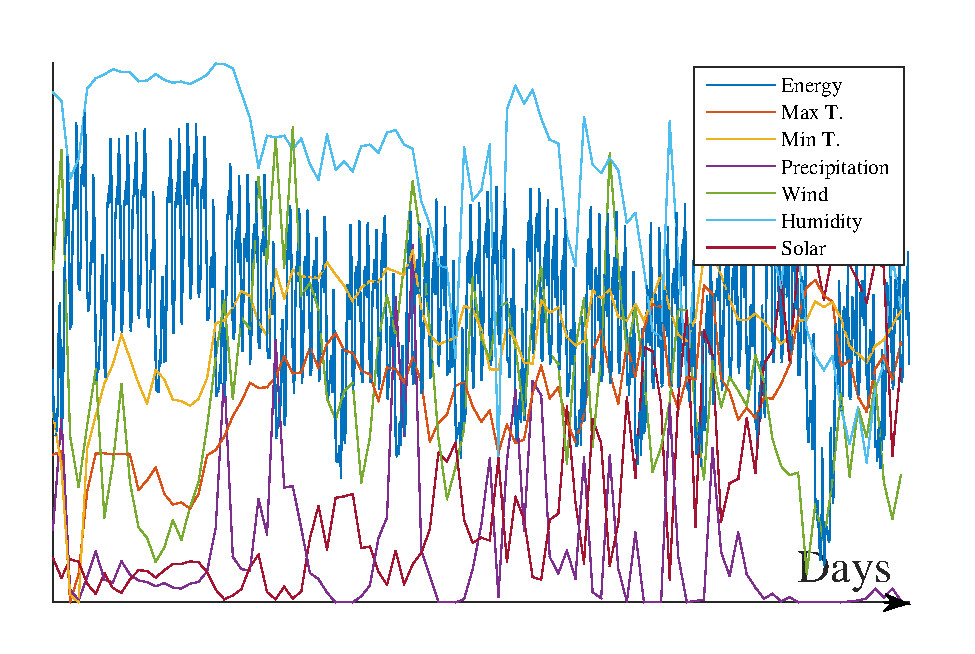
\includegraphics[width=0.55\textwidth]{data_example_100days.eps}
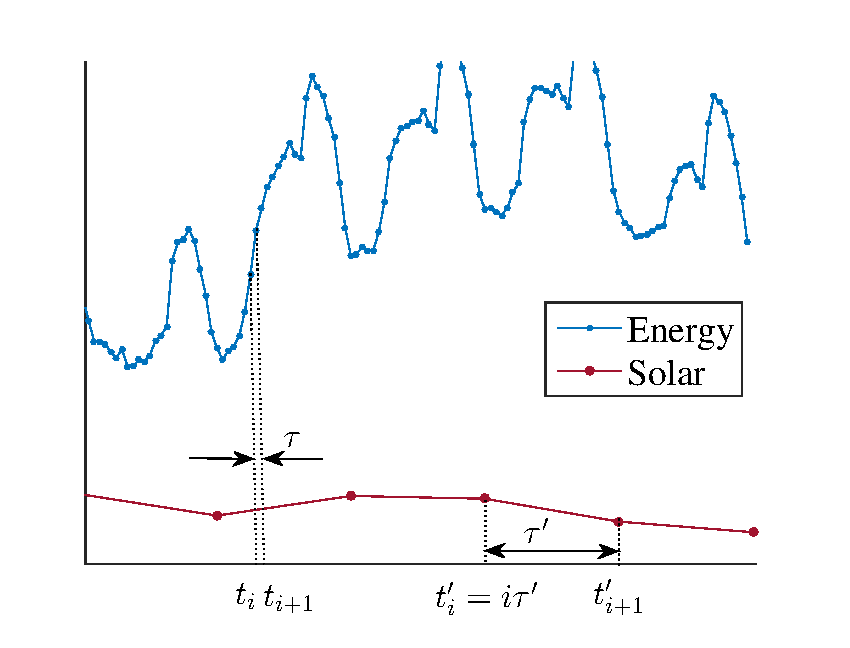
\includegraphics[width=0.5\textwidth]{data_sampling_100days.eps}

\end{frame}
%-----------------------------------------------------------------------------------------------------
\begin{frame}{Time series forecasting}

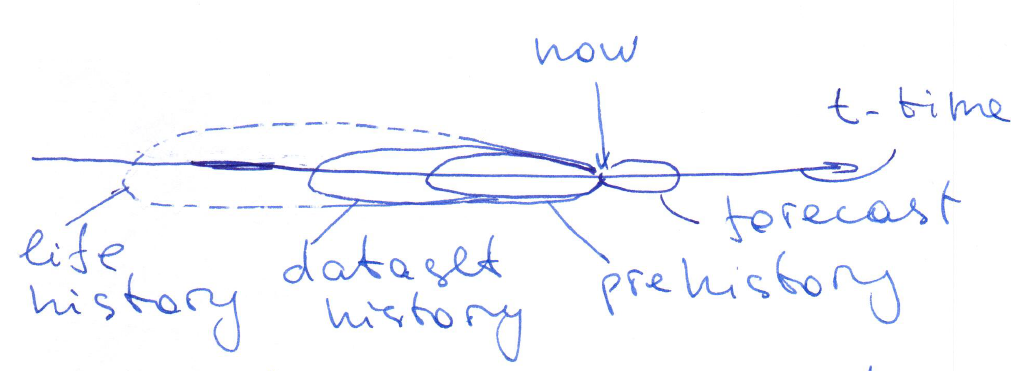
\includegraphics[width=0.9\textwidth]{online_forecasting_paradigm.png} \\

%\includegraphics[trim= 2cm 0 0 15cm,clip,width=0.5\textwidth]{feature_selection/EnergyWeather/res_orig_test_Min_Temperature_MSVR_fs_SSA.png}

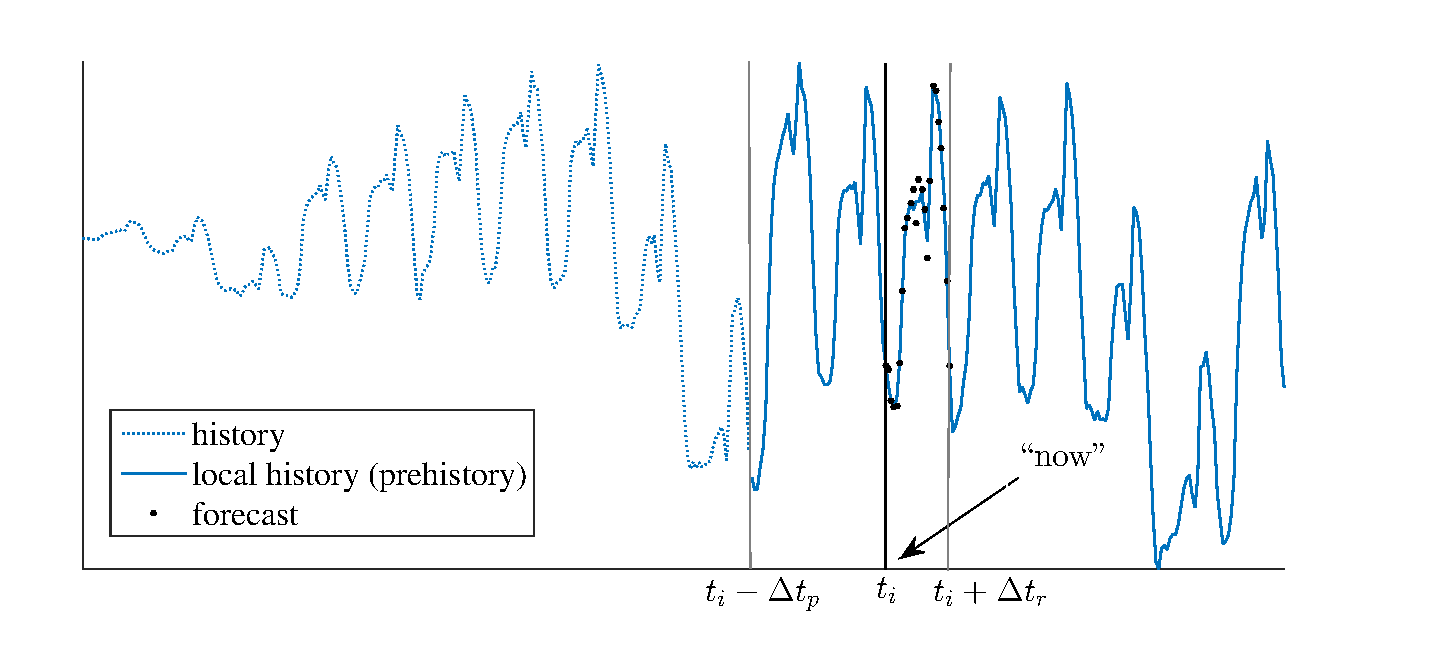
\includegraphics[width=0.9\textwidth]{history_prehistory_frc.eps}


\end{frame}
%-----------------------------------------------------------------------------------------------------
\begin{frame}{Design matrix}

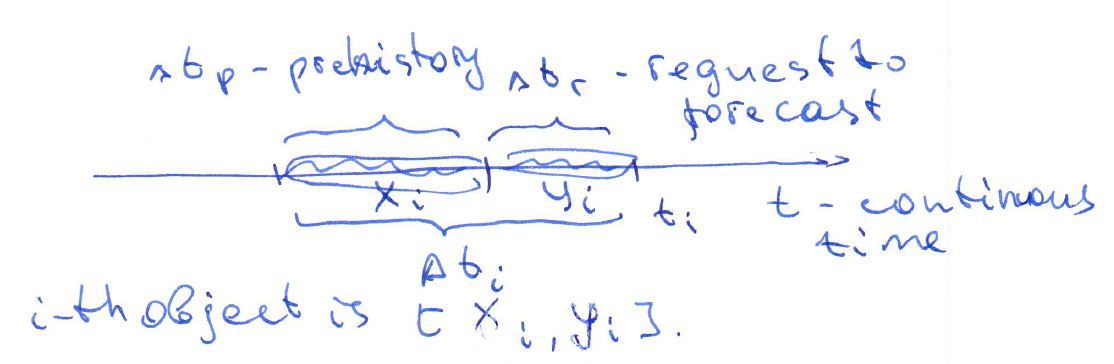
\includegraphics[width=0.9\textwidth]{draw_object.png} \\

\[
[\bx_i | \by_i] = \underbrace{s(t_i-\dtr-\dtp),\dots,}_{\bx_i} \underbrace{s(t_i-\dtr),\dots,s(t_i))}_{\by_i}. \]

\end{frame}
%-----------------------------------------------------------------------------------------------------
\begin{frame}{Design matrix}


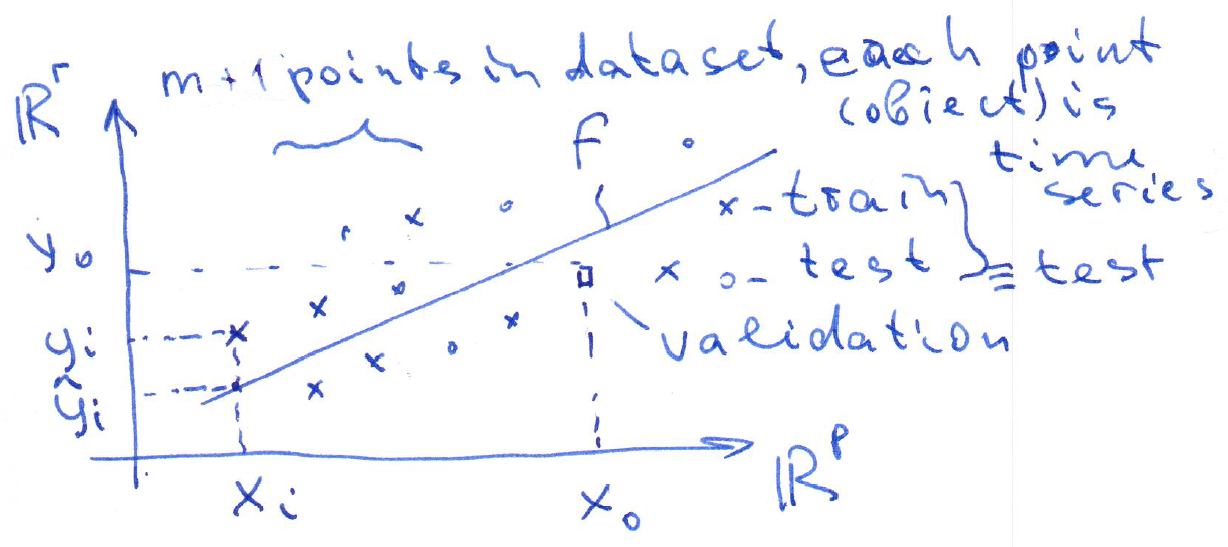
\includegraphics[width=0.9\textwidth]{forecasting_model.png}

\[
\bX^*= \left[
\begin{array}{c|c}
\underset{1{\times}n}{\x} & \underset{1{\times}r}{{\by}}  \\
\hline
 \underset{m{\times}n}\bX & \underset{m{\times}r}\bY  \\
 %\hline
 \end{array}
\right] =  \left[
\begin{array}{lll|lll}
\bx^{(1)} & \dots & \bx^{(Q)} & \by^{(1)} &  \dots & {\by}^{(Q)}   \\
\hline
\bx_m^{(1)}  & \dots & \bx_m^{(Q)} & \by_m^{(1)} &  \dots & \by_m^{(Q)}   \\
\vdots & \ddots & \vdots & \vdots & \ddots & \vdots  \\
\bx_1^{(1)} & \dots & \bx_1^{(Q)} & \by_1^{(1)}  & \dots & \by_1^{(Q)}   \\


\end{array}
\right]. \]

\end{frame}
%-----------------------------------------------------------------------------------------------------
%\begin{frame}{Design matrix}
%
%\centering{
%\includegraphics[width=0.5\textwidth]{fig/feature_selection/EnergyWeather/generation_orig_test_fs_NW.eps}
%}
%
%\end{frame}
%-----------------------------------------------------------------------------------------------------
\begin{frame}{Regression problem}

Now we are able to state the regression problem as follows:
\begin{equation}\label{eq:regression_problem}
\hat{\y} = f(\x, \hat{\w}), ~\hat{\w} = \argmin_{\hat{\w}}S\bigl(\bw|\fx(\bw,\bx),\by\bigr). %\text{~where~}
\end{equation}

Here the error function $S\bigl(\bw|\fx(\bw,\bx),\by\bigr)$ averages forecasting errors of  $[\x_i | \by_i]$  over all segments $i = 1, \dots, m$ in the test set:
\[ S\bigl(\bw|\fx(\bw,\bx),\by\bigr) = \frac{r}{m}\sum_{i=1}^{m} l(\y_i, f(\x_i, \w)).\]

Let $\veps$ denote residual vector
\[ \veps = [\varepsilon_1, \dots, \varepsilon_r] = \by - \hat{\by}\]
for the forecast $\hat{\by} = \fx(\bw,\bx)$ of $\by$.


\end{frame}
%-----------------------------------------------------------------------------------------------------
\begin{frame}{Types of forecasting errors}

\Wider[4em]{
\begin{itemize}
\item scale-dependent metrics: mean
absolute error
\vspace{-1em}
\[ MAE = \frac{1}{r}\sum_{j = 1}^{r} |\varepsilon_j|,\]
\vspace{-1em}
\item percentage-error metrics: (symmetric) mean absolute percent error
\vspace{-1em}
\[ MAPE = \frac{1}{r}\sum_{j = 1}^{r} \frac{|\varepsilon_j|}{|y_j|}, \quad sMAPE = \frac{1}{r}\sum_{j = 1}^{r} \frac{2|{\varepsilon}_j|}{|\hat{y}_j + y_j|}, \]
\vspace{-1em}
\item relative-error metrics (to residues $\veps^{*}$ of a benchmark method):
\vspace{-1em}
 \[ MRAE = \frac{1}{r}\sum_{j = 1}^{r} \frac{|{\varepsilon}_j|}{{\varepsilon}^{*}_j},\]
 \vspace{-1em}
\item and
scale-free error metrics:
\vspace{-1em}
\[ MASE = \frac{n-1}{r}\frac{\sum_{i=1}^r|\varepsilon_j|}{\sum_{j=2}^n |x_j - x_{j-1}|}. \]
\end{itemize}
}
\end{frame}
%-----------------------------------------------------------------------------------------------------
\begin{frame}{Rolling validation}

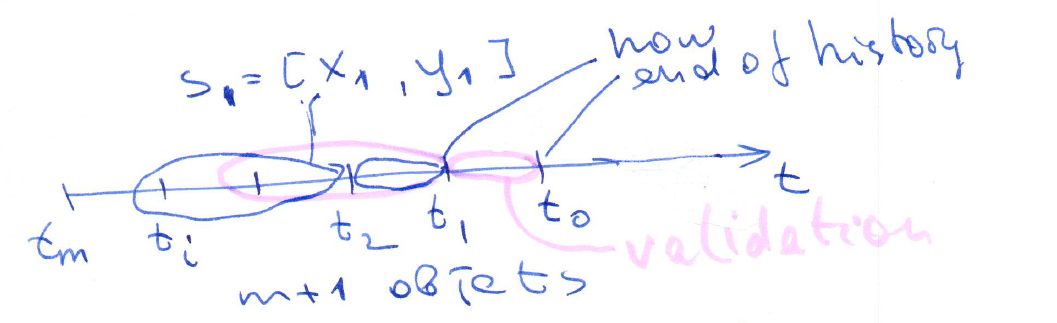
\includegraphics[width=0.9\textwidth]{design_matrix_generation.png}

%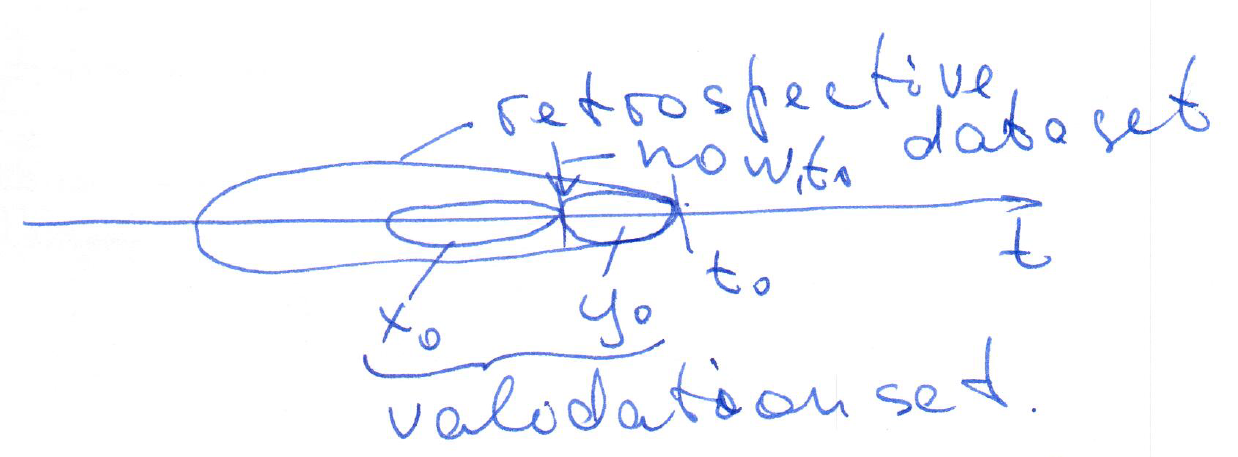
\includegraphics[width=\textwidth]{retrospective_validation.png}

\end{frame}
%-----------------------------------------------------------------------------------------------------
\begin{frame}{Rolling validation}

\begin{enumerate}[1)]
\item construct the validation vector $\bx^*_{\text{val},k}$ for time series of the length~$\dtr$ as the first row of the design matrix~$\bZ$,
\item construct the rest rows of the design matrix~$\bZ$ for the time after~$t_k$ and present it as
 \[\bZ = \left[\begin{array}{c|c}
 \dots & \dots \\
 \hline
 \underset{1{\times}n}{\bx_{\text{val}, k}} & \underset{1{\times}r}{\by_{\text{val}, k}}  \\
 \hdashline
 \underset{m_{\min}{\times}n}{\bX_{\text{train}, k}}  & \underset{m_{\min}{\times}r}{\bY_{\text{train}, k}} \\
 \hline
 \dots & \dots \\
 \end{array}\right], \Big{\uparrow}_{k}
 \]
\item optimize model parameters~$\bw$ using~$\bX_{\text{train}, k}, \bY_{\text{train}, k}$,
\item compute residues~$\veps_k = \by_{\text{val}, k} - \fx(\bx_{\text{val}_k}, \bw)$ and $\text{MAPE}$,
\item increment $k$ and repeat.
\end{enumerate}

\end{frame}
%-----------------------------------------------------------------------------------------------------
\begin{frame}
\vfill
\begin{center}
{\Large \bf Feature generation}
\end{center}
\vfill
\end{frame}
%-----------------------------------------------------------------------------------------------------
\begin{frame}{Generating extra features}

To augment feature description, consider the following types of features:
\begin{enumerate}[1)]
\item the local history of all time series themselves,
\item transformations (non-parametric and parametric) of local history,
\item parameters of the local models,
\item distances to the centroids of local clusters.
\end{enumerate}

\end{frame}
%-----------------------------------------------------------------------------------------------------
\begin{frame}{Functional transforms}

The procedure of generating new features $\vf$ requires:
\begin{itemize}
\item the original features $\bx = \{\bx_1, \dots, \bx_Q\}$,
\item the set of primitive functions $G = \{g(\mathbf{b},\bx)\}$,
    $$g:\bx \mapsto \vf;$$
\item the generation rules: $\mathcal{G}\supset G$, where the superposition $g_k\circ g_l \in \mathcal{G}$ w.r.t. numbers and types of the input and output arguments;
\item the simplification rules: $g_u$ is not in $\mathcal{G}$, if there exist a rule
$$
r:g_u \mapsto g_v \in \mathcal{G}.
$$
\end{itemize}


\bigskip
The result is
\begin{itemize}
\item[] the set of the features $\bx=\{\mathbf{x}_1,\dots,\mathbf{x}_{Q},\vf_{1},\dots,\vf_N\}.$
%where
%$$
%y^i=\frac{1}{1+\exp\left(-\sum\limits_{j\in\mathcal{A}\subseteq\mathcal{J}} w_j\mathbf{x}^i_j\right)}.
%$$
\end{itemize}

\end{frame}
%-----------------------------------------------------------------------------------------------------
\begin{frame}{Examples of nonparametric transformation functions}

\begin{itemize}
\item Univariate \quad
\begin{tabular}{c|c}
Formula		&	Output dimension	\\ \hline
$	\sqrt{x}	$	&	1		\\ \hline
$	x\sqrt{x}	$	&	1		\\ \hline
$	\arctan{x}	$	&	1		\\ \hline
$	\ln{x}	$	&	1	\\ \hline
$	x\ln{x}	$	&	1	\\
\end{tabular}

\medskip
\item Bivariate \quad
\begin{tabular}{c|c}
Plus	&	$	x_1 + x_2	$	\\ \hline
Minus	&	$	x_1 - x_2	$	\\ \hline
Product	&	$	x_1 \cdot x_2	$	\\ \hline
Division	&	$	\frac{x_1}{x_2}	$	\\ \hline
	&	$	x_1\sqrt{x_2}	$	\\ \hline
	&	$	x_1\ln{x_2}	$	\\
\end{tabular}

\end{itemize}

\end{frame}
%-----------------------------------------------------------------------------------------------------
\begin{frame}{Nonparametric transformations: sample statistics}

Nonparametric transformations include basic data statistics:
\begin{itemize}
\item Sum or average value of each row $\bx_i$, $i = 1, \dots, m$:
\[ \vf_i = \sum_{j = 1}^{n} x_{ij}, \text{~or~} \vf'_i = \frac{1}{n}\sum_{j=1}^{n} x_{ij}. \]

\item Min and max values: $ \vf_i = \min_{j} x_{ij}$, $\vf'_i = \max_{j} x_{ij} $.
\item Standard deviation: \[\vf_i = \frac{1}{n-1}\sqrt{\sum_{j=1}^{n}(x_{ij} - \text{mean}(\bx_i))^2}.\]
\item Data quantiles: $ \vf_{i}  = [X_1, \dots, X_K], $
where \[\sum_{j=1}^{n} [X_{k-1} < x_{ij} \leq X_k ] = \frac{1}{K}, \text{~for~} k = 1,\dots, K. \]
\end{itemize}

%\renewcommand*{\arraystretch}{1.3}
%\begin{tabular}{|p{90pt}|c|p{50pt}|p{50pt}|p{50pt}|p{60pt}|}
%\hline
%sum	&	$	\sum_i x_i	$		\\ \hline
%mean	&	$	(\sum_i x_i)/m	$	\\ \hline
%min	&	$	\min_i x_i	$		\\ \hline
%max	&	$	\max_i x_i	$		\\ \hline
%std	&	$	\frac{1}{m-1}\sqrt{\sum_i(x_i - \text{mean}(x))^2}	$		\\ \hline
%hist &	$	\sum_i [X_{j-1} < x_i \leq X_j ]	$	\\ \hline
%conv &	$	\sum_j x_{i-j}w_j 	$	&	1	&	 \leq m$	\\
%\end{tabular}

\end{frame}
%-----------------------------------------------------------------------------------------------------
\begin{frame}{Nonparametric transformations: Haar's transform}

\Wider[2em]{
Applying Haar's transform produces multiscale representations of the same data.

\medskip

Assume that $n = 2^{K}$ and init $\vf_{i,j}^{(0)} = \vf_{i,j}'^{(0)} = x_{ij}$ for $j = 1, \dots, n$.

To obtain coarse-graining and fine-graining of the input feature vector $\bx_i$,  for $k = 1, \dots, K$ repeat:
\begin{itemize}
\item data averaging step \[\vf_{i,j}^{(k)} =  \frac{\vf_{i, 2j-1}^{(k-1)} + \vf_{i, 2j}^{(k-1)}}{2}, \quad j=1, \dots, \frac{n}{2^k}, \]
\item and data differencing step \[\vf_{i,j}'^{(k)} =  \frac{\vf_{i, 2j}'^{(k-1)} - \vf_{i, 2j-1}'^{(k-1)}}{2}, \quad j=1, \dots, \frac{n}{2^k}. \]


\end{itemize}
The resulting multiscale feature vectors are~$\vf_i = [\vf_i^{(1)}, \dots, \vf_i^{(K)}]$ and
$\vf'_i = [\vf_i'^{(1)}, \dots, \vf_i'^{(K)}]$.

 }
\end{frame}
%-----------------------------------------------------------------------------------------------------
\begin{frame}{Parametric transformations}

Optimization of the transformation function parameters~$\bb$ is iterative:

\begin{enumerate}
\item Fix the vector~$\hat\bb$, collected over all the primitive functions~$\{g\}$, which generate features~$\vf$:
\[
\hat\bw = \arg\min S\bigl(\bw|\fx(\bw,\bx),\by\bigr),\quad
\text{where}
\quad \vf(\hat\bb,\bs) \subseteq \bx.
\]

\item Optimize transformation parameters~$\hat\bb$ given model parameters~$\hat{\bw}$
\[
\hat\bb = \arg\min S\bigl(\bb|\fx(\hat\bw,\bx),\by\bigr).
\]
\end{enumerate}
Repeat these steps until vectors~$\hat\bw,\hat\bb$ converge.

\end{frame}
%-----------------------------------------------------------------------------------------------------
\begin{frame}{Examples of parametric transformation functions}

\Wider[4em]{
\begin{tabular}{p{65pt}|c|p{30pt}|p{20pt}|p{20pt}}
Function name	&		Formula		&	Output dim.	&	Num. of args	&	Num. of pars	\\ \hline
Add constant	&	$	x + w	$	&	1	&	1	&	1	\\ \hline
Quadratic	&	$	w_2 x^2 + w_1 x + w_0	$	&	1	&	1	&	3	\\ \hline
Cubic	&	$	w_3x^3 + w_2 x^2 + w_1 x + w_0	$	&	1	&	1	&	4	\\ \hline
%Nonparametric sin	&	$	\sin(x)	$	&	1	&	1	&	0	\\ \hline
%Sin	&	$	\sin(w_0 + w_1x)	$	&	1	&	1	&	2	\\ \hline
%Square root	&	$	\sqrt{x}, \;x\sqrt{x}	$	&	1	&	1	&	0	\\ \hline
%Arctangent	&	$	\arctan{x}	$	&	1	&	1	&	0	\\ \hline
%Logarithmic	&	$	\ln{x}, \;x\ln{x}	$	&	1	&	1	&	0	\\ \hline
Logarithmic sigmoid	&	$	1/(w_0 + \exp(-w_1x))	$	&	1	&	1	&	2	\\ \hline
Exponent	&	$	\exp{x}	$	&	1	&	1	&	0	\\ \hline
Normal	&	$	\frac{1}{w_1\sqrt{2\pi}}\exp\left(\frac{(x-w_2)^2}{2w_1^2}\right)	$	&	1	&	1	&	2	\\ \hline
Multiply by constant	&	$	x\cdot w	$	&	1	&	1	&	1	\\ \hline
Monomial	&	$	w_1 x^{w_2}	$	&	1	&	1	&	2	\\ \hline
Weibull-2	&	$	w_1w_2x^{w_2-1}\exp{-w_1x^{w_2}}	$	&	1	&	1	&	2	\\ \hline
Weibull-3	&	$	w_1w_2x^{w_2-1}\exp{-w_1(x-w_3)^{w_2}}	$	&	1	&	1	&	3	\\ \hline
\dots & \dots & \dots & \dots & \dots \\
\end{tabular}
}

\end{frame}
%-----------------------------------------------------------------------------------------------------
\begin{frame}{Monotone functions}

\Wider[2em]{
\begin{itemize}
\item \textbf{By grow rate} \\
\begin{tabular}{p{90pt}|c|c}
Function name	&		Formula	&	Constraints	\\ \hline
Linear	&	$	w_1 x + w_0	$	&		\\ \hline
Exponential rate	&	$	\exp(w_1x + w_0)	$	&		$w_1 > 0$	\\ \hline
Polynomial rate	&	$	\exp(w_1\ln x + w_0)	$	&		$w_1 > 1$	\\ \hline
Sublinear polynomial rate	&	$\exp(w_1\ln x + w_0)$		&	$0 < w_1 < 1$	\\ \hline
Logarithmic rate	&	$	w_1\ln x + w_0	$	&	$w_1 > 0$	\\ \hline
Slow convergence	&	$	w_0 + w_1/x	$	&	$w_1 \neq 0$	\\ \hline
Fast convergence	&	$	w_0 + w_1\cdot\exp(-x)	$	&	$w_1 \neq 0 $	\\
\end{tabular}

\item \textbf{Other}  \\
\begin{tabular}{p{90pt}|c|c}
Soft ReLu & $\ln(1+e^{x}) $	&			\\ \hline
Sigmoid	&	$	1/(w_0 + \exp(-w_1x))	$	&		$w_1 > 0$	\\ \hline
Softmax	&	$	1/(1 + \exp(-x))	$	& \\ \hline
Hiberbolic tangent	&	$	\tanh(x)	$	&	 	\\ \hline
% &   $-1,\text{~for~} x < -1$ &		&		&		&		\\
%hardtan &  $0, \text{~if~} -1\leq x\leq 1, $ &	1	&	1	&	0	&		\\
% &  $1,\text{~for~} x > 1$ &		&		&		&		\\ \hline
softsign & $\frac{|x|}{1+|x|}$	&	\\
\end{tabular}
\end{itemize}
}

\end{frame}
%-----------------------------------------------------------------------------------------------------
\begin{frame}{Parameters of the local models}

Other options:
\begin{itemize}
\item Parameters of SSA approximation of the time series $\bx^{(q)}$.
\item  Parameters of the FFT of each $\bx^{(q)}$.
\item Parameters of polynomial/spline approximation of each $\bx^{(q)}$.
\end{itemize}

\end{frame}
%-----------------------------------------------------------------------------------------------------
\begin{frame}{Parameters of the local models: SSA}

For the time series~$\bs$ construct the Hankel matrix with a~period~$k$ and shift~$p$, so~that for~$\bs = [s_1,\dots,s_T]$ the matrix
\[
\bH^* =
\left[ \begin{array}{c|cc}
s_T  & \dots & s_{T-k+1} \\
\vdots & \ddots & \vdots \\
s_{k+p} & \dots & s_{1+p}\\
s_k & \dots & s_1 \\
\end{array}
\right],
\text{~where~} 1\geqslant p \geqslant k .
\]
Reconstruct the regression to the first column of the matrix~$\bH^*=[\bh, \bH]$ and denote its least square parameters as the feature vector
\[
\boldsymbol{\phi}(\bs) = \arg\min \| \bh-\bH \boldsymbol{\phi}\|_2^2.
\]
For the orignal feature vector~$\bx = [\bx^{(1)}, \bx^{(Q)}]$ use the parameters $\boldsymbol{\phi}(\bx^{(q)})$, $q = 1, \dots, Q$ as the features.

\end{frame}
%-----------------------------------------------------------------------------------------------------
\begin{frame}{Metric features: distances to the centroids of local clusters}

Apply kernel trick to the time series.

\begin{enumerate}
\item For given local feature vector~$\bx_i^{(q)}$, $q=1,\dots, Q$ compute $k$-means centroids~$\bc_p^{(m)}$, $p = 1, \dots, P$.
\item   With the selected $k$-means distance function~$\rho$ construct the feature vector
\[
\vf_i^{(q)} = [\rho(\bc_1^{(q)},\bx_i^{(q)}),\dots,\rho(\bc^{(q)}_P,\bx_i^{(q)})] \in \R_+^P.
\]
\end{enumerate}
%This $k$-means of another clustering procedure may use internal parameters, so that there are no parameters to be included to the feature vector or to the forecasting model.

\bigskip

The procedure may be applied to each $\bx^{(q)}$ or directly to the $\bx = [\bx^{(1)}, \dots, \bx^{(Q)}]$, resulting in only $P$ additional features instead of $Q\cdot{P}$
\end{frame}
%-----------------------------------------------------------------------------------------------------
\begin{frame}
\vfill
\begin{center}
{\Large \bf Feature selection}
\end{center}
\vfill
\end{frame}
%-----------------------------------------------------------------------------------------------------
\begin{frame}
\vfill
\begin{center}
{\Large \bf Mixture models}
\end{center}
\vfill
\end{frame}
%-----------------------------------------------------------------------------------------------------
%\begin{frame}{Mixture models}
%
%Let $D = (X, \by)$ denote the data, where $X = [\bx_1\T, \dots, \bx_i, \dots, \bx_m\T]\T$,
% denotes the inputs $\bx_i\in\R^{n}$, $\by$ denotes the targets $y_i \in Y$. The task is to estimate $y_i$, given $\bx_i$. Assuming linear model $f$ with gaussian noise
% \[
% y = f(\x, \w) + \varepsilon, ~ f(\x, \w) = \w\T\x, \; \varepsilon \sim \mathcal{N}(0,\beta) \Rightarrow y \sim \mathcal{N}(\w\T\x, \beta),
% \]
% obtain the maximum likelihood estimate
% \[\hat{y} = \hat{\w}\T\x, ~ \hat{\w} = \argmax_{\w} \frac{1}{2\beta}\sum_{i=1}^{m}(y_i - \w\T \x_i)^2 \]
% for the output.
%
%% Maximum likelihood estimation gives
%%\[ \hat{y} = \argmax_{y in Y} P(y|\bx, \w).\]
%\end{frame}
%-----------------------------------------------------------------------------------------------------
\begin{frame}{Linear mixture models}%{EM-algorithm for mixture models}
Assume the target variable $\by$ is generated by one of~$K$ linear models $f_{k}(\x, \w_k)$. Let the distribution of the target variable~$\by$ be a mixture of normal distributions
\[
p(\by|\x, \bth) = \sum_{k=1}^{K}\pi_k\;\mathcal{N}(\by|\w_k\T\bx,\beta) = \]
\[ \sum_{k=1}^K
\frac{1}{(2\pi\beta_k)^{n/2}} \exp \left(
( -\frac{1}{2\beta_k}(\by - \w_k\T X)^{\top}(\by - \w_k\T X) \right).
\]
Here~$\bth$ denotes the concatenated vector of parameters:
\[
\bth = [\w_1,\dots,\w_k,\boldsymbol{\pi},\beta]\T,
\]
where $\boldsymbol{\pi} = [\pi_1,\dots,\pi_k]$ are weights of the models,
and $\bB = \beta \bI_m$ is the covariance matrix for~$\by$.


\end{frame}
%-----------------------------------------------------------------------------------------------------
\begin{frame}{Parameter estimation}

\Wider[2em]{
To find maximum likelihood estimates of $\hat{\bth}$
\[
\hat{\bth} = \argmax_{\bth}\ln p(\by|\bth),
%~\ln p(\by|\bth) = \sum_{i=1}^{m}\ln\left( \sum_{k=1}^K  \pi_k\mathcal{N}(\by|\w\T_{k}\x_i,\beta) \right).
\]

introduce hidden indicator variables~$Z = \left[\bz_1,\dots,\bz_m\right], \quad z_{ik}\in \{0,1\},$ such that
\[z_{ik} = 1 \Leftrightarrow y_i\sim\mathcal{N}(\w_k\T\x_i, \beta).\]
Then the loglikelihood function $p(\by, Z|X, \bth)$ takes the form
\[p(\by|X, Z, \bth) = \sum_{i=1}^{m}\sum_{k=1}^{K} z_{ik} \left( \ln\pi_k + \ln\mathcal{N}(y_i|\w\T_{k}\x_i,\beta) \right). \]

%\[=\sum_{i=1}^{m}\sum_{k=1}^{K} z_{ik} \left( \ln\pi_k - \frac{1}{2\beta}(y_i-\w\T_{k}\x_i)^2 + \frac{n\ln{\beta}}{2} + \text{const}\right).\]
\bigskip

\textbf{EM-algorithm:} instead of $p(\by|X, \bth)$ maximize the expected loglikelihood $\mathsf{E}_{Z} [p(\y, Z|X, \bth)]$ of the observed data.
%\[\mathsf{E}_{Z} [p(\y, Z|X, \bth)] = \]
%\[ \sum_{i=1}^{m}\sum_{k=1}^{K} \gamma_{ik} \Big( \ln\pi_k - \frac{1}{2\beta}(y_i-\w\T_{k}\x_i)^2 +
%  \frac{n\ln{\beta}}{2}\Big),\] where $\gamma_{ik} = \mathsf{E}[z_{ik}|\y, X]$.
}
\end{frame}
%-----------------------------------------------------------------------------------------------------
\begin{frame}{Expectation step}
\Wider[3em]{
Expectation-Maximization algorithm maximizes $\mathsf{E}_{Z} [p(\y, Z|X, \bth)]$, updating parameters estimates $\textcolor{red}{\bth^{(r+1)}}$ in two iterative steps with $\textcolor{blue}{\bth^{(r)}}$ fixed.

\vspace{2em}

{\bf E-step}: obtain $\mathsf{E}(Z) = [\gamma_{ik}]$. Using Bayesian rule, obtain:
\[
\textcolor{red}{\gamma_{ik}^{(r+1)}} = \mathsf{E}(z_{ik}) = p(k|\x_i, \textcolor{blue}{\bth^{(r)}}) =
    \frac{
        \textcolor{blue}{\pi_k}\mathcal{N}(y_i|\x_i\T\textcolor{blue}{\w^{(r)}_{k}}, \textcolor{blue}{\beta^{(r)}})
        }{
        \sum_{k'=1}^{K}\textcolor{blue}{\pi_{k'}}\mathcal{N}(y_i|\x_i\T\textcolor{blue}{\w^{(r)}_{k'}}, \textcolor{blue}{\beta^{(r)}}).
        } \]

Define expectations of joint loglikelihood $\ln p(\y, Z|X, \bth)$ with respect to the posteriors distribution~$p(Z|\y,\bth)$
\[
Q^{(r)}(\bth) = \mathsf{E}_Z(\ln p(\y, Z|\bth)) = \sum_{i=1}^m\sum_{k=1}^K\gamma_{ik}^{(r+1)}\left(
        \ln\pi^{(r)}_k+\ln\mathcal{N}(y_i|\x_i\T\w^{(r)}_{k},\beta^{(r)})
    \right).
\]
}

\end{frame}
%-----------------------------------------------------------------------------------------------------
\begin{frame}{Maximization step}

\Wider[2em]{
Expectation-Maximization algorithm maximizes $\mathsf{E}_{Z} [p(\y, Z|X, \bth)]$, updating parameters estimates $\textcolor{red}{\bth^{(r+1)}}$ in two iterative steps with $\textcolor{blue}{\bth^{(r)}}$ fixed.

\vspace{2em}


{\bf M-step:} update parameters $\bth$, maximizing $Q^{(r)}(\bth) = \mathsf{E}_Z(\ln p(\y, Z|\bth))$ with respect to~$\bth$ with~$\textcolor{blue}{\gamma^{(r+1)}}$ fixed:

\[
\textcolor{red}{\pi^{(r+1)}_k} = \frac{1}{n}\sum_{i=1}^m { \textcolor{blue}{\gamma_{ik}^{(r+1)}}}.
\]

\[
\textcolor{red}{\w^{(r+1)}_k} = \argmax_{\w_k}\sum_{i=1}^m -\textcolor{blue}{\gamma^{(r+1)}_{ik}}
    \left(
        y_i-\w_k\T\x_i
    \right)^2,
\]
\[
\beta^{(r+1)}_k = \argmax_{\beta}\sum_{i=1}^m\gamma^{(r+1)}_{ik}
    \left(n\ln\beta
        -\frac{1}{\beta}(y_i-\x_i\T\w^{(r+1)}_k)^2
    \right).
\]
}
\end{frame}
%-----------------------------------------------------------------------------------------------------
\begin{frame}{Maximization step}

\Wider[2em]{
Expectation-Maximization algorithm maximizes $\mathsf{E}_{Z} [p(\y, Z|X, \bth)]$, updating parameters estimates $\textcolor{red}{\bth^{(r+1)}}$ in two iterative steps with $\textcolor{blue}{\bth^{(r)}}$ fixed.

\vspace{2em}


{\bf M-step:} update parameters $\bth$, maximizing $Q^{(r)}(\bth) = \mathsf{E}_Z(\ln p(\y, Z|\bth))$ with respect to~$\bth$ with~$\textcolor{blue}{\gamma^{(r+1)}}$ fixed:

\[
\pi^{(r+1)}_k = \frac{1}{n}\sum_{i=1}^m { \gamma_{ik}^{(r+1)}}.
\]

\[
\textcolor{blue}{\w^{(r+1)}_k} = \argmax_{\w_k}\sum_{i=1}^m -\gamma^{(r+1)}_{ik}
    \left(
        y_i-\w_k\T\x_i
    \right)^2,
\]
\[
\textcolor{red}{\beta^{(r+1)}_k} = \argmax_{\beta}\sum_{i=1}^m\textcolor{blue}{\gamma^{(r+1)}_{ik}}
    \left(n\ln\beta
        -\frac{1}{\beta}(y_i-\x_i\T\textcolor{blue}{\w^{(r+1)}_k})^2
    \right).
\]
}
\end{frame}
%-----------------------------------------------------------------------------------------------------
%\begin{frame}
%\vfill
%\begin{center}
%{\Large \bf Mixture of Experts}
%\end{center}
%\vfill
%
%\end{frame}
%-----------------------------------------------------------------------------------------------------
\begin{frame}{Mixture of Experts}

Suppose that each model $f(\x, \w_k)$ generates a sample $(\x, y)$ with some probability $p(k|\x, \w)$. Then
the following factorization holds
\begin{equation*}\label{eq:mixture_of_experts} p(y|\x, \bth) = \sum_{k=1}^{K} p(y, k| \x, \bth) = \sum_{k=1}^{K} p(k|\x, \bth)p(y|k, \x, \bth)\end{equation*}
 for $p(y|\x, \bth)$.

 \bigskip

 Here $p(k|\x, \bth)$ correspond to weight parameters $\pi_k$ in mixture models dependent on the inputs $\x$:
\[\pi_k(\x, \bv_k) = \frac{\exp(\bv_k\T\x)}{\sum_{k'=1}^K \exp(\bv_{k'}\T\x)}.\]

\medskip

Parameter's estimation via EM differs only in M-step.



\end{frame}
%-----------------------------------------------------------------------------------------------------
\begin{frame}{EM for Mixture of experts}

\Wider[1em]{

\textbf{E-step}: compute hidden variables $\textcolor{blue}{\gamma^{(r+1)}_{ik}}$, the expectation of the indicator
variables, as previously shown.

\medskip

\textbf{M-step}: find new parameter estimates
   \[ \textcolor{red}{\bv^{(r+1)}_k }= \argmax_{\bv} \sum_{i=1}^m \textcolor{blue}{\gamma_{ik}^{(r+1)}}\ln\pi_k(\x_i, \bv), \quad\quad \]

  \[   \textcolor{red}{\w^{(r+1)}_k} = \argmax_{\w_k} \left[- \sum_{i=1}^m\textcolor{blue}{\gamma^{(r+1)}_{ik}}
    \left(
        y_i-\w_k\T\x_i
    \right)^2 \right], \]

  \[ \beta^{(r+1)}_k = \argmax_{\beta} \left[ n\ln\beta
        -\frac{1}{\beta}\left(y_i-\x_i\T\w^{(r+1)}_k\right)^2 \right]. \]

}
\end{frame}
%-----------------------------------------------------------------------------------------------------
\begin{frame}{EM for Mixture of experts}

\Wider[1em]{

\textbf{E-step}: compute hidden variables $\textcolor{blue}{{\gamma^{(r+1)}_{ik}}}$, the expectation of the indicator
variables, as previously shown.

\medskip

\textbf{M-step}: find new parameter estimates
   \[ \bv^{(r+1)}_k = \argmax_{\bv} \sum_{i=1}^m \gamma_{ik}^{(r+1)}\ln\pi_k(\x_i, \bv), \quad\quad \]

  \[   \textcolor{blue}{\w^{(r+1)}_k} = \argmax_{\w_k} \left[- \sum_{i=1}^m\gamma^{(r+1)}_{ik}
    \left(
        y_i-\w_k\T\x_i
    \right)^2 \right], \]

  \[ \textcolor{red}{\beta^{(r+1)}_k} = \argmax_{\beta} \left[ n\ln\beta
        -\frac{1}{\beta}\left(y_i-\x_i\T\textcolor{blue}{\w^{(r+1)}_k}\right)^2 \right]. \]

}
\end{frame}

%-----------------------------------------------------------------------------------------------------
\begin{frame}
\vfill
\begin{center}
{\Large \bf Computational experiments}
\end{center}
\vfill

\end{frame}
%-----------------------------------------------------------------------------------------------------
%\begin{frame}{Experimental setting}
%
%\begin{tabular}{p{3cm}|c}
%Datasets & 6 \\
%Time series in each dataset & 7 \\
%Models & 4 \\
%Feature combinations & 9 \\
%Loss functions & 6 \\
%\end{tabular}
%
%\end{frame}
%-----------------------------------------------------------------------------------------------------
\begin{frame}{Data}
\Wider[3em]{
\textbf{1.} Original Polish electricity load time series, 1999--2004, including:
\begin{itemize}
\item hourly energy time series (total of 52512 observations),
\item six daily weather time series from Warsaw (2188 observations): Max Temperature, Min Temperature,
Precipitation, Wind, Relative Humidity, Solar.
\end{itemize}
\textbf{2--5.} Data sets with artificial inserted missing values, 1, 3, 5 and 10\% missing. \\
\textbf{6.} Data set with artificially varied sampling rate.

\centering{
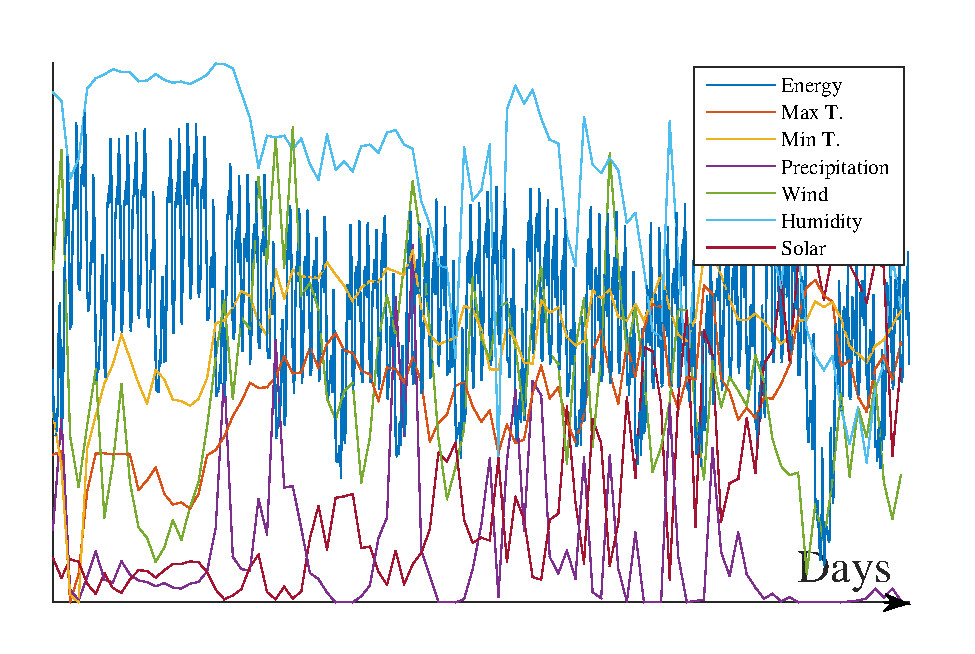
\includegraphics[width=0.56\textwidth]{data_example_100days.eps}}

}

\end{frame}
%-----------------------------------------------------------------------------------------------------
\begin{frame}{Data}

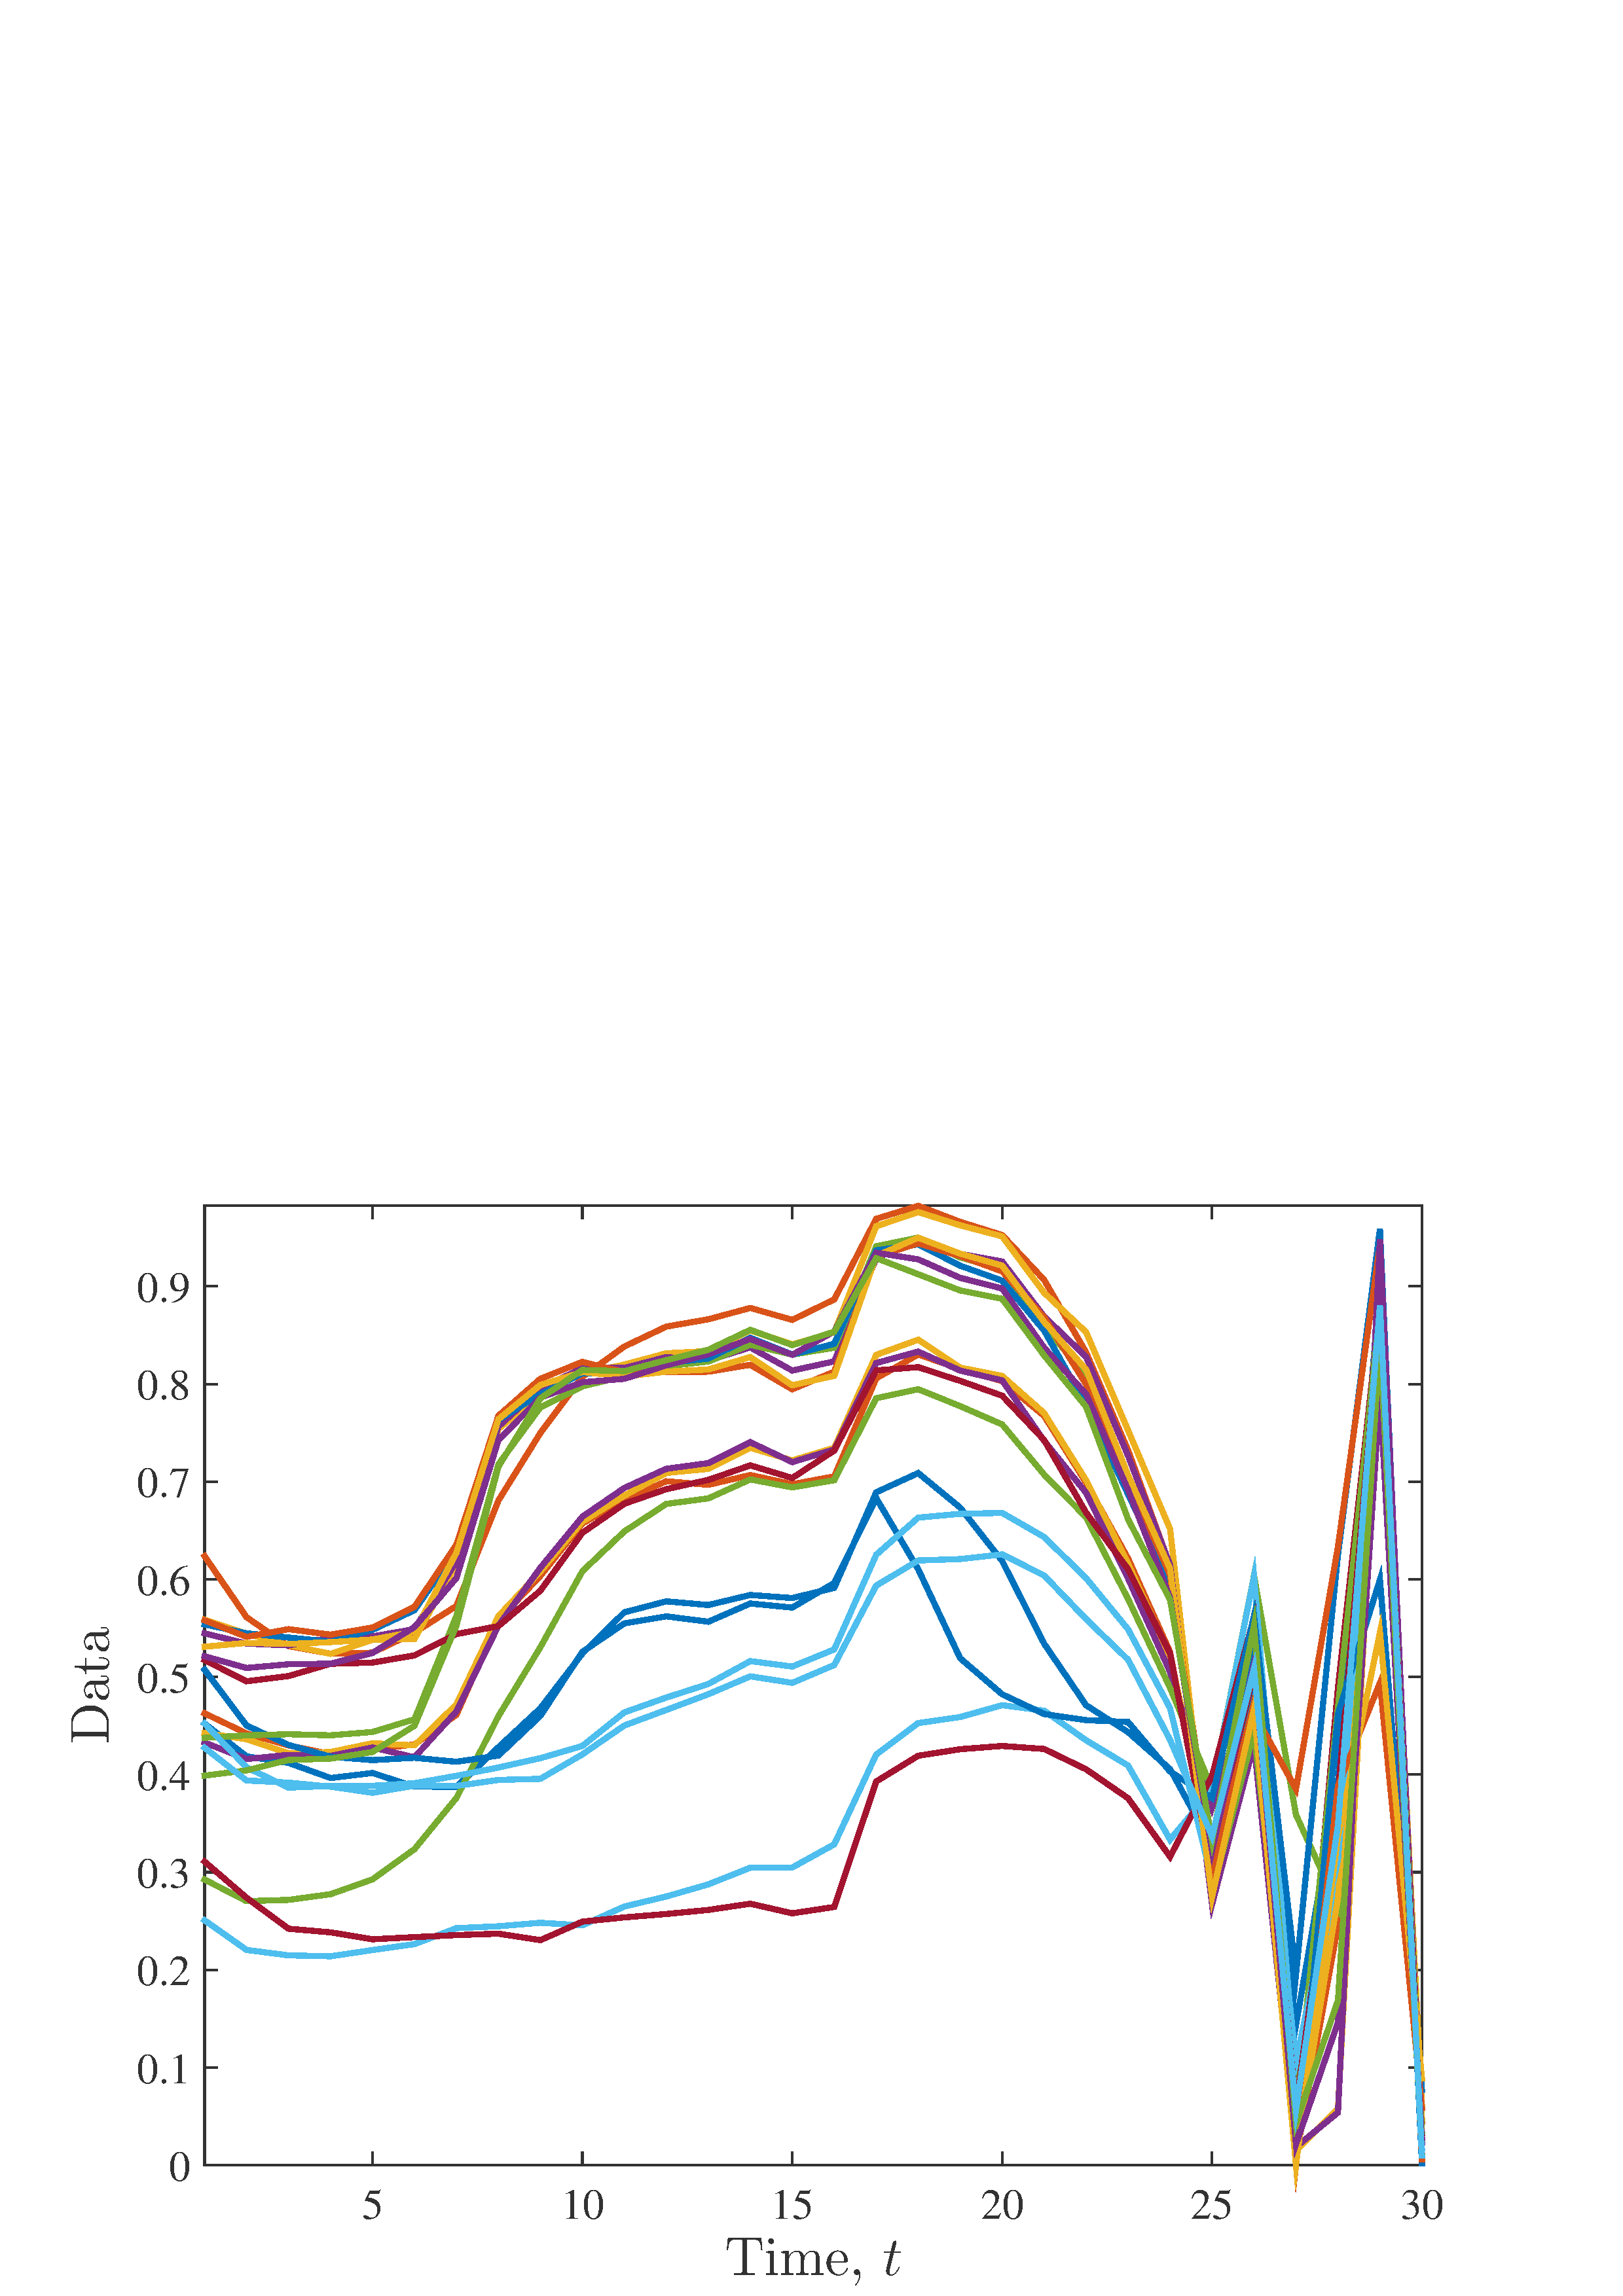
\includegraphics[trim= 2cm 0 0 15cm,clip,width=0.5\textwidth]{fig/feature_selection/EnergyWeather/data_segms_orig_test.png}
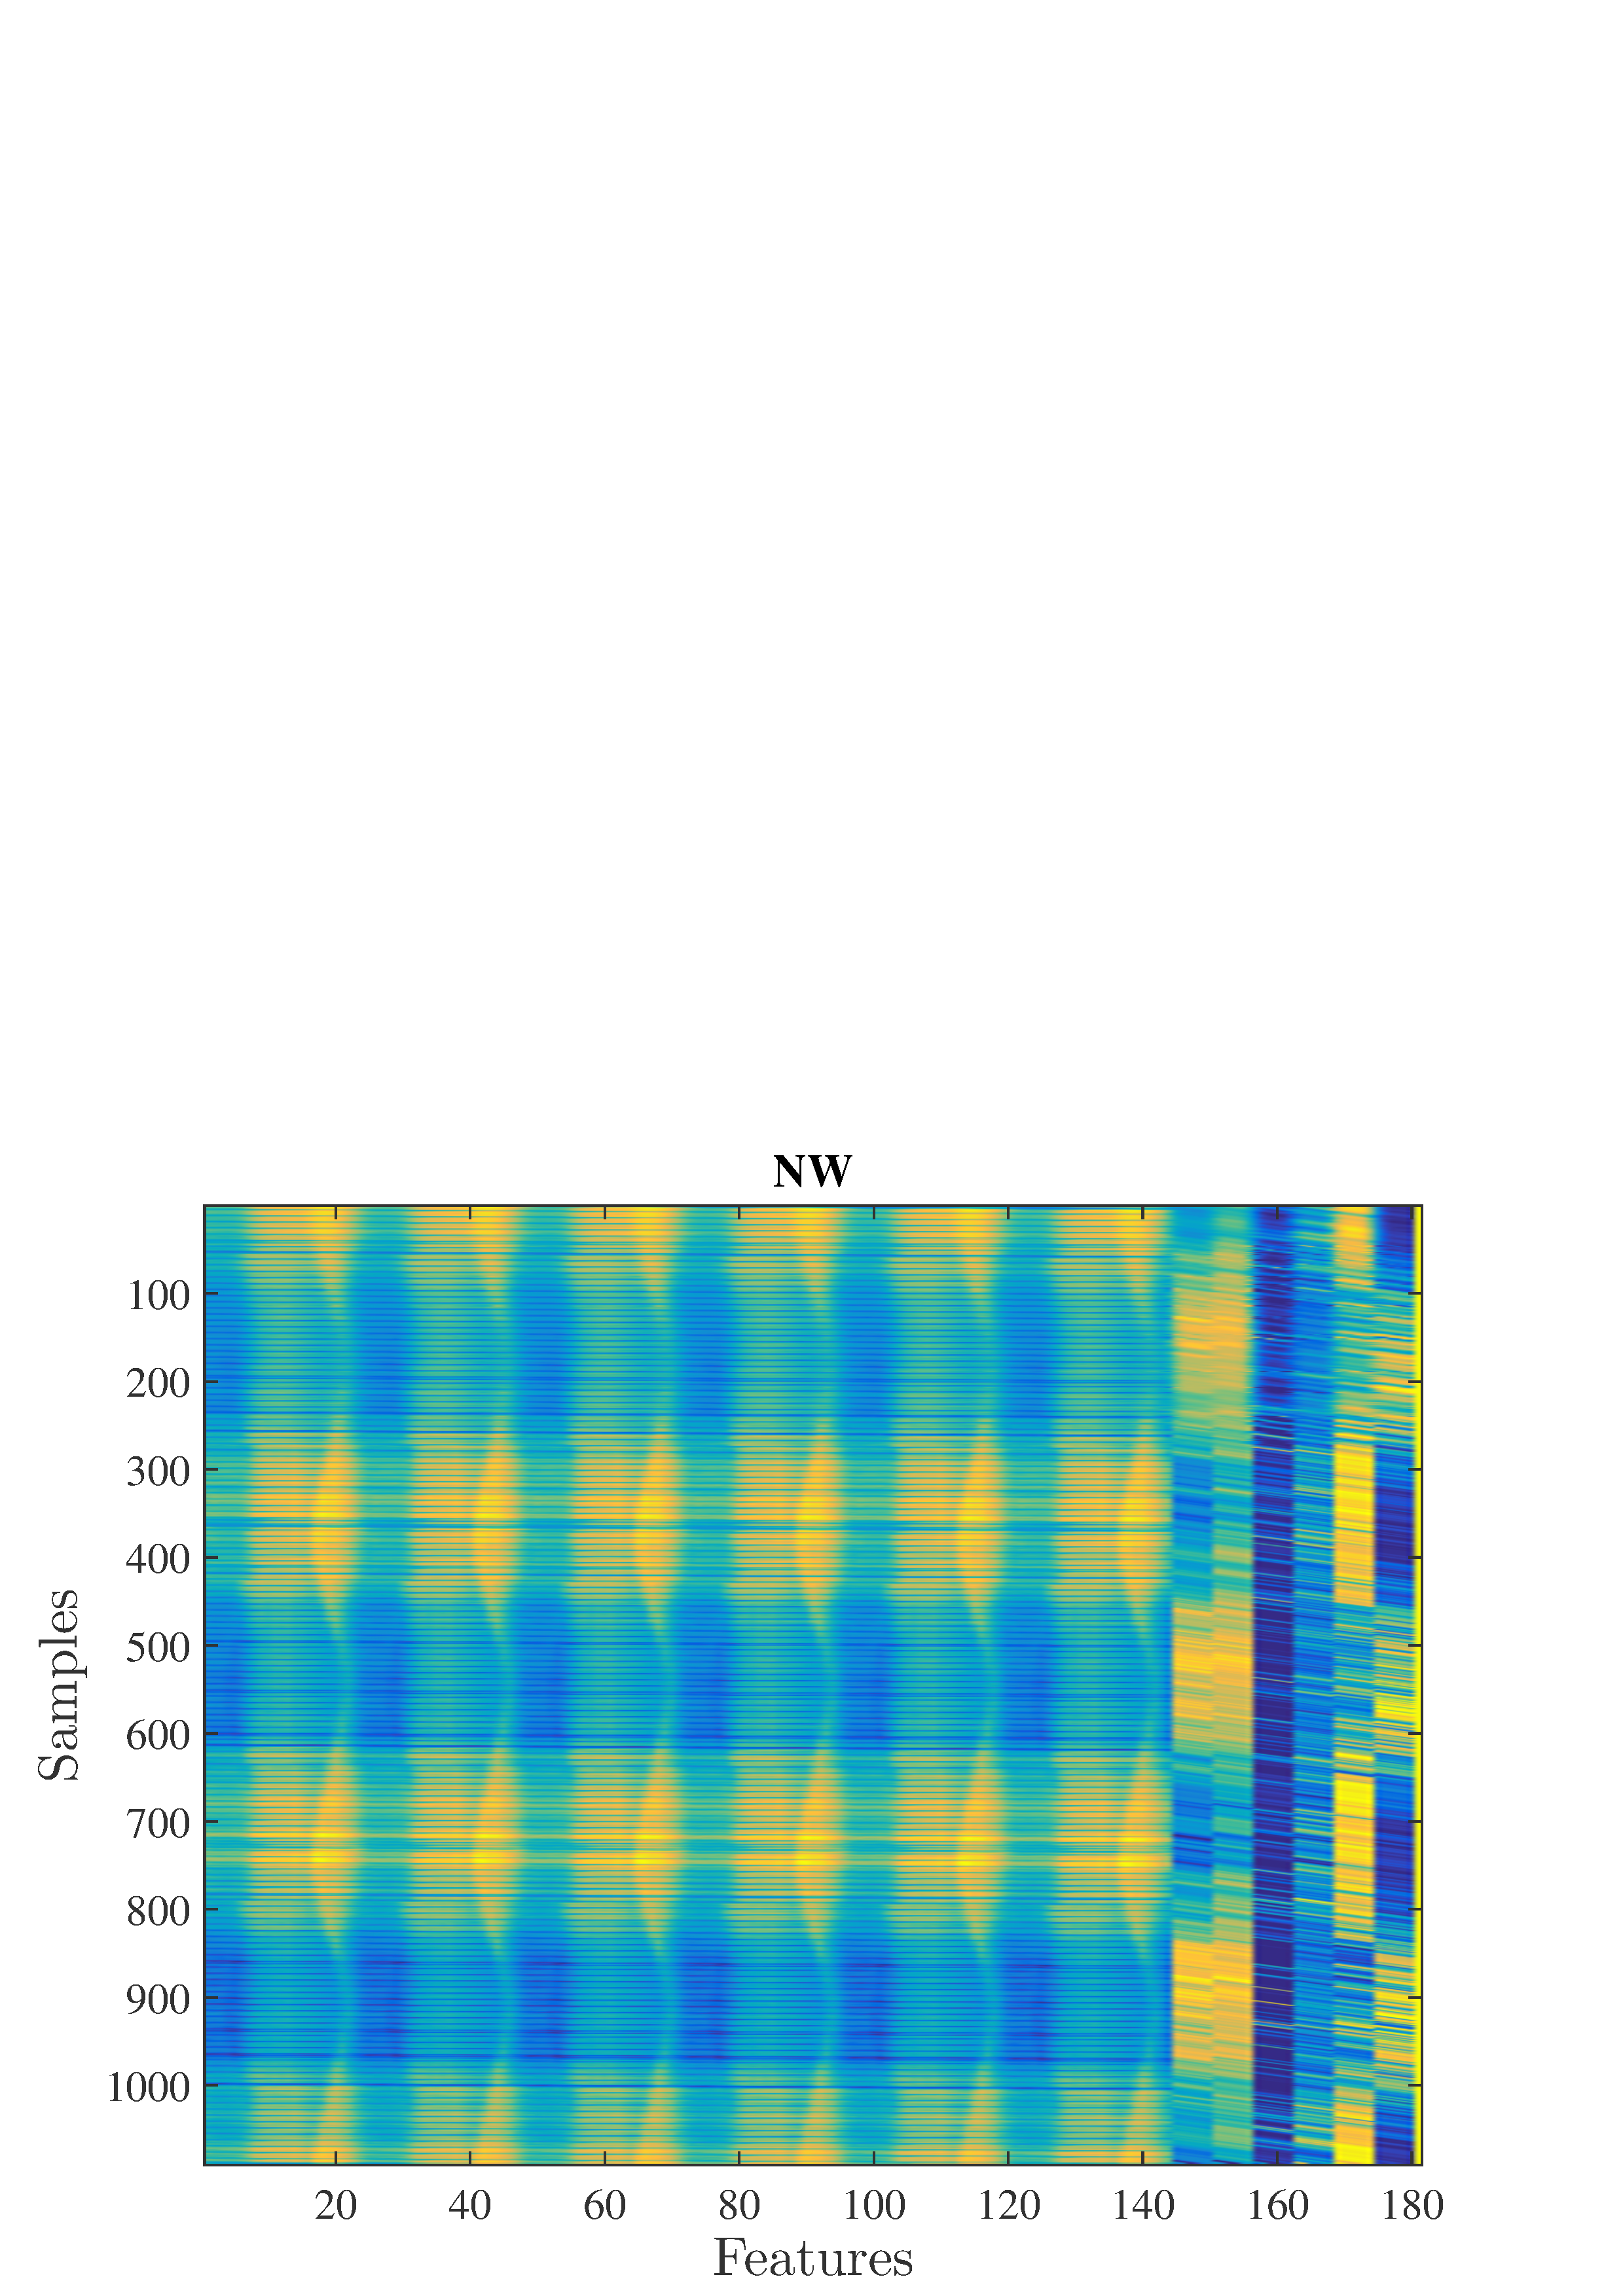
\includegraphics[trim= 2cm 0 0 15cm,clip,width=0.5\textwidth]{fig/feature_selection/EnergyWeather/generation_orig_test_fs_NW.png}

\quad Target variables. \hspace{3cm} The design matrix.

\end{frame}
%-----------------------------------------------------------------------------------------------------
\begin{frame}{Models and features}
\Wider[3em]{
\textbf{Models:}
\begin{itemize}
\item  Baseline method: $\hat{s}_i = s_{i-1}$.
\item  Multivariate linear regression (MLR) with $l_2$-regularization. Regularization coefficient: 2 \\
\item SVR with multiple output. Kernel type: RBF, $p_1$: 2, $p_2$: 0, $\gamma$: 0.5, $\lambda$: 4.
\item Feed-forward ANN with single hidden layer, size: 25 \\
\item Random forest (RF). Number of trees: 25 , number of variables for each decision split: 48.
\end{itemize}


\medskip

\textbf{Feature combinations:}
\begin{itemize}
\item History: the standard regression-based forecast with no additional features.
\item SSA, Cubic, Conv, Centroids, NW: history + a particular feature.
%: parameters of local SSA approximation, ``Cubic'': coefficients of cubic polynomial approximation, ``Conv'': for multiscale features and sample statistics, ``Centroids'':  metric distances to centroids.
\item All: all of the above, with no feature selection.
\item  PCA and NPCA: all generation strategies with feature selection.
\end{itemize}
}
\end{frame}
%-----------------------------------------------------------------------------------------------------
\begin{frame}{Forecasting errors, SMAPE}
\Wider[4em]{
\begin{tabular}{|p{1cm}|c|c|c|c|c|c|c|c|}
\hline
Data &Energy & Max T. & Min T. & Precip. & Wind & Humid. & Solar\\
\hline
\multicolumn{8}{|c|}{Test} \\
\hline
\multirow{1}{*}{orig} &   0.111 &    0.127 &    0.111 &    1.222 &    0.396 &    0.201 &    0.495\\
\cline{1-7}
\hline
\multirow{1}{*}{0.01} &   0.230 &    0.185 &    0.129 &    1.028 &    0.397 &    0.254 &    0.577\\
\cline{1-7}
\hline
\multirow{1}{*}{0.03} &   0.231 &    0.191 &    0.137 &    1.026 &    0.396 &    0.253 &    0.591\\
\cline{1-7}
\hline
\multirow{1}{*}{0.05} &   0.230 &    0.200 &    0.141 &    1.017 &    0.390 &    0.250 &    0.592\\
\cline{1-7}
\hline
\multirow{1}{*}{0.1} &   0.247 &    0.198 &    0.151 &    1.192 &    0.381 &    0.225 &    0.562\\
\cline{1-7}
\hline
\multirow{1}{*}{varying} &   0.124 &    0.139 &    0.102 &    1.232 &    0.395 &    0.219 &    0.489\\
\cline{1-7}
\hline
\hline
\multicolumn{8}{|c|}{Train} \\
\hline
\multirow{1}{*}{orig} &   0.031 &    0.073 &    0.057 &    0.848 &    0.111 &    0.051 &    0.267\\
\cline{1-7}
\hline
\multirow{1}{*}{0.01} &   0.034 &    0.055 &    0.040 &    0.595 &    0.111 &    0.055 &    0.253\\
\cline{1-7}
\hline
\multirow{1}{*}{0.03} &   0.034 &    0.057 &    0.042 &    0.595 &    0.110 &    0.055 &    0.249\\
\cline{1-7}
\hline
\multirow{1}{*}{0.05} &   0.034 &    0.060 &    0.043 &    0.592 &    0.109 &    0.054 &    0.246\\
\cline{1-7}
\hline
\multirow{1}{*}{0.1} &   0.031 &    0.081 &    0.063 &    0.743 &    0.102 &    0.051 &    0.272\\
\cline{1-7}
\hline
\multirow{1}{*}{varying} &   0.027 &    0.057 &    0.044 &    0.888 &    0.112 &    0.055 &    0.272\\
\cline{1-7}
\hline
\end{tabular}
}

\end{frame}
%-----------------------------------------------------------------------------------------------------
\begin{frame}{Feature analysis}

\centering{
\includegraphics[width=0.6\textwidth]{fig/feature_selection/EnergyWeather/best_models_all_colormatrix.eps}
}

Ratio of times each combination of model and feature performed best for at least one of the time series (7) or error functions (6), all (6) data sets ($ 6\times 7\times 6 = 252$  cases).

\end{frame}
%-----------------------------------------------------------------------------------------------------
\begin{frame}{Validation of multiple forecast approach}

Additional loss functions: mean residues (test/train), standard deviation of residues (test/train) $\rightarrow$ 6 loss functions.

\centering{
\includegraphics[width=0.6\textwidth]{fig/feature_selection/EnergyWeather/improvement_all_colormatrix.eps}
}

Ratio of datasets, where best forecasts outperformed baseline according to a particular error function.

\end{frame}
%-----------------------------------------------------------------------------------------------------
\begin{frame}
\vfill
\begin{center}
{\Large \bf Resampling time series}
\end{center}
\vfill
\end{frame}
%-----------------------------------------------------------------------------------------------------
\begin{frame}{Resampling time series}

Suppose that the observations $s_i = s(t_i)$ of the signal $s(t)$ are sampled unevenly:
\[\Gs = \{t_1, \dots, t_T\}, \quad t_i \neq i\cdot\frac{t_T - t_1}{T-1} \]

\bigskip

To obtain evenly spaced observations:
\begin{enumerate}[1)]
\item select a new sampling rate $\trs$,
\item form the new grid
\[\Grs = \{t_1, \dots, \Trs \}, \quad t_i  = t_1 + (i-1)\cdot\trs \]
\item and approximate
unobserved evenly-spaced values $\hat{s_i} = s(t_i)$, $t_i \in \Grs$ using the sampled observations $s_i = s(t_i)$, $t_i \in \Gs$.
\end{enumerate}

\end{frame}
%-----------------------------------------------------------------------------------------------------
\begin{frame}{Resampling: special case}

\begin{enumerate}
\item The initial sampling rate is approximately even, but distortions are possible:
\[ t_i = i\cdot\tau + \delta_i, |\delta_i| < \frac{\tau}{2}.\]
In this case the number $\Ts$ of resampled observations equals the initial number of observations $T$.
\end{enumerate}

\centering{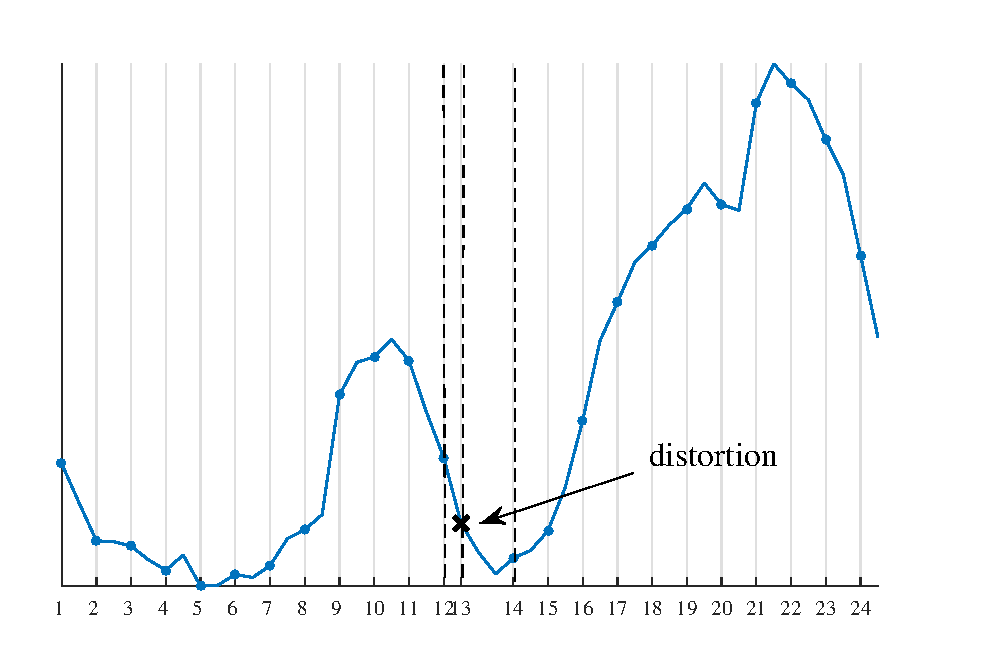
\includegraphics[width=0.6\textwidth]{data_resampling_distortions.eps}}


\end{frame}
%-----------------------------------------------------------------------------------------------------
\begin{frame}{Resampling: special case}

\begin{enumerate}
\item[2.] The sampling rate is even, but some values are missing:
\[ |t_{i+1} - t_{i}| = n\tau, n \in \mathbb{N}.\]
Here $\ts = \tau$ and missing values are the only ones that one needs to approximate.
\end{enumerate}

\centering{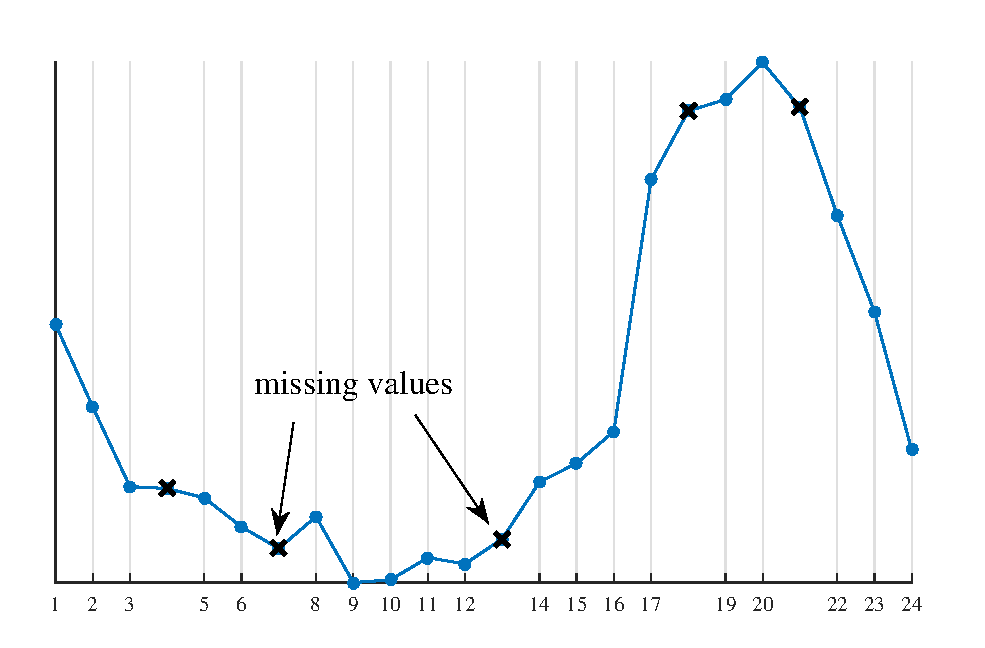
\includegraphics[width=0.7\textwidth]{data_resampling_missing_values.eps}}


\end{frame}
%-----------------------------------------------------------------------------------------------------
\begin{frame}{Resampling: special case}

\Wider[3em]{
\begin{enumerate}
\item[3.] Time series $\bs$ comprises a finite number of intervals $\bs_k$, each sampled from $s(t)$ at fixed sampling rate:
\[ \bs = \left[s(\tau_1), \dots, s(T_1\tau_1), s(T_1\tau_1 + \tau_2), \dots,  s\left(\sum_{k}T_k\tau_k\right)\right], \] where $\sum_k{T_k} = T.$
Here we select the maximum sampling rate $\fs = \max_{k} \frac{1}{\tau_k}$ and upsample the rest time series, using piecewise constant approximation.
\end{enumerate}

\centering{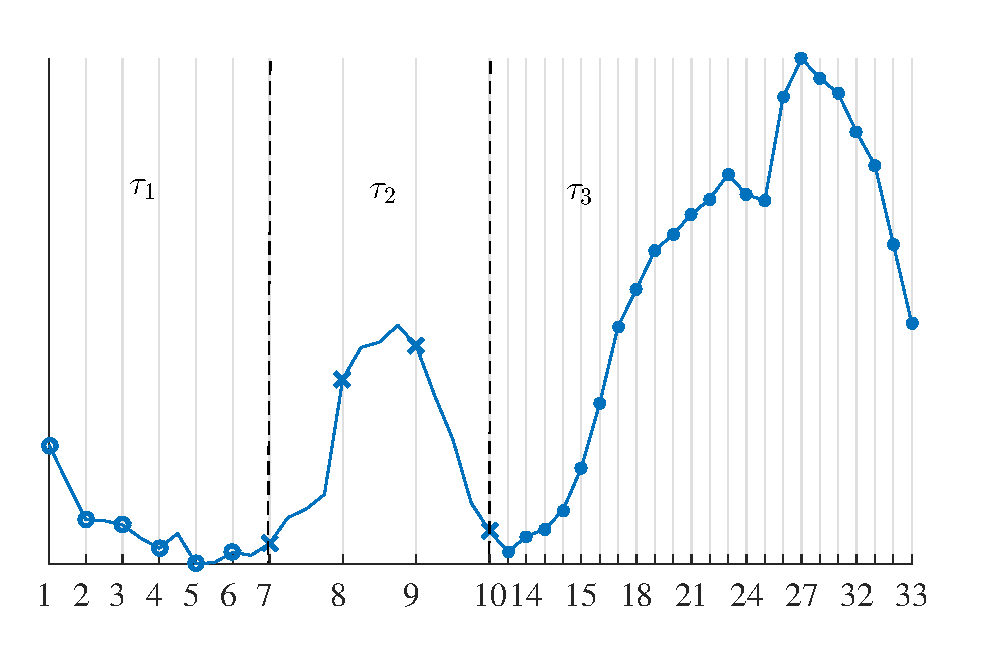
\includegraphics[width=0.5\textwidth]{data_resampling_varying_rates.eps}}


}

\end{frame}
%-----------------------------------------------------------------------------------------------------
\begin{frame}{Resampling details}

Suppose that the signal $s(t)$ is bandlimited with frequency $\fb$.

\bigskip

\textbf{Nyquist–Shannon  sampling condition:} it is sufficient to sample the signal $s(t)$ with frequency
\[ \frac{1}{\trs} = \fs > 2\fb\]
to be able to fully reconstruct the signal from its discretely sampled observations $s(t_i) = s(i\ts)$.

\bigskip

%For $\fs > 2\fb$, Whittaker-Shannon interpolation
%\[s(t) = \sum_{i = -\infty}^{\infty} s_i\text{sinc}\left(\frac{t-i\ts}{\ts}\right)\]
%of the time series $\bs$ yields perfect reconstruction of the signal $s(t)$.
%
%\medskip

Discrete signals are never bandlimited %Sampling with $\fs < 2\fb$ causes distortions known as aliasing
$\Rightarrow$ the time series have to be low-pass filtered to satisfy the Nyquist condition.


\end{frame}
%-----------------------------------------------------------------------------------------------------
\begin{frame}{Upsampling procedure}

Let $\Grs$ be the desired grid, $G \subseteq \Grs$. To obtain $s(\Grs)$:
\begin{enumerate}
\item Approximate $s(\Grs\setminus G)$ using piecewise linear approximation.
%\item Lowpass filter $\bs$, so that $\bs$ is bendlimited with $\fb$. \\
\item Find $\bs$'s FFT coefficients $a_j,\; b_j$ for  $j = 1, \dots, 2^{\lfloor\log_2T\rfloor}$.
\item Set $a_j = 0,\; b_j=0$, for  $j > 2^{{\lfloor\log_2T\rfloor} - 1}$.
\item Reconstruct the time series, using inverse FFT.

\end{enumerate}
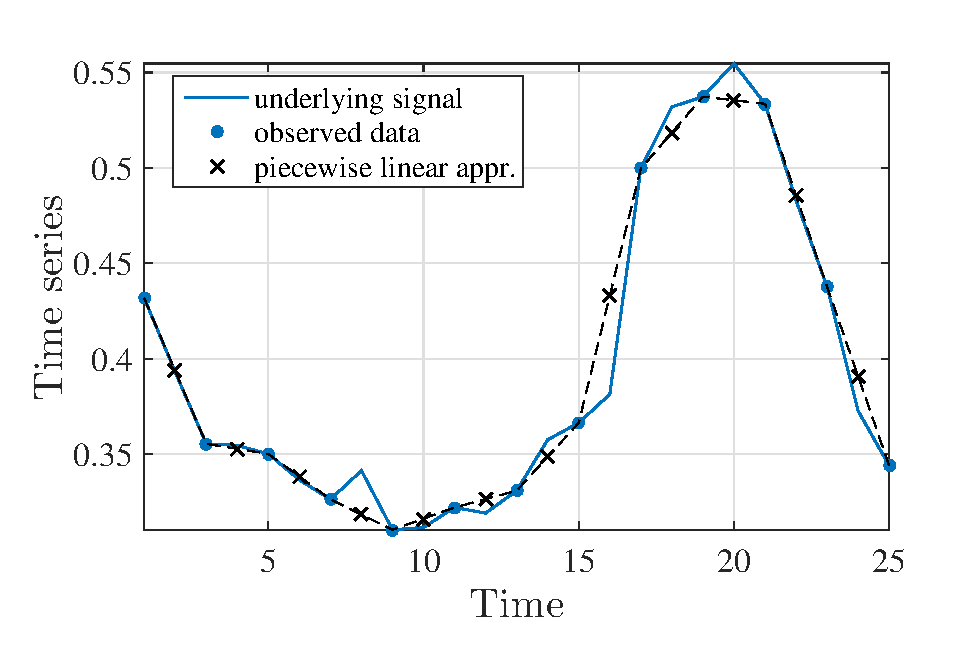
\includegraphics[width=0.55\textwidth]{pw_linear_approximation.eps}
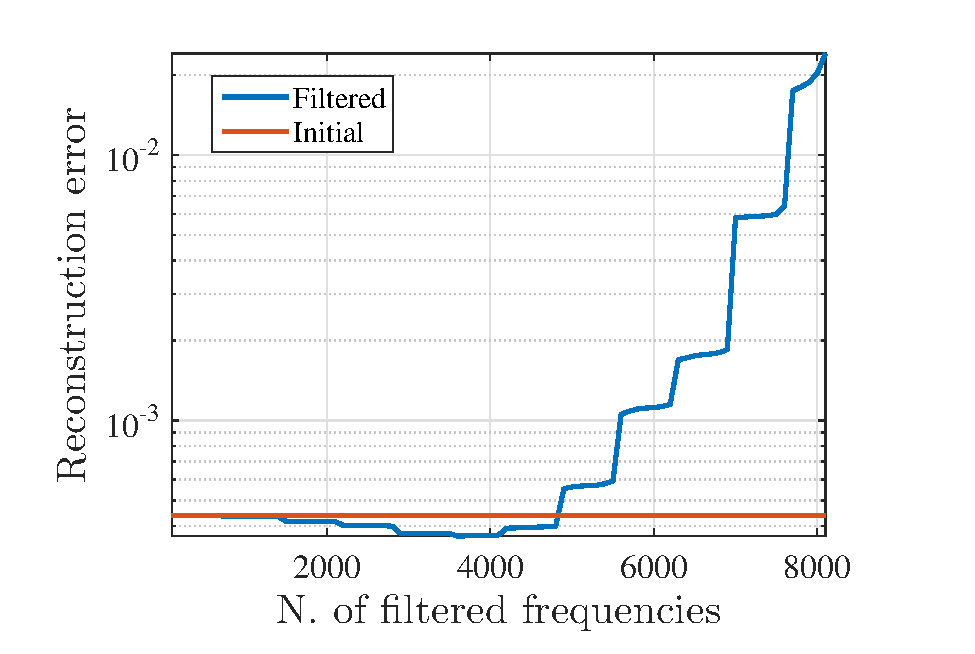
\includegraphics[width=0.55\textwidth]{fft_rec_err_upsampling.eps}

\end{frame}
%-----------------------------------------------------------------------------------------------------
\begin{frame}{Resampling}


Piece-wise constant approximation of missing values:
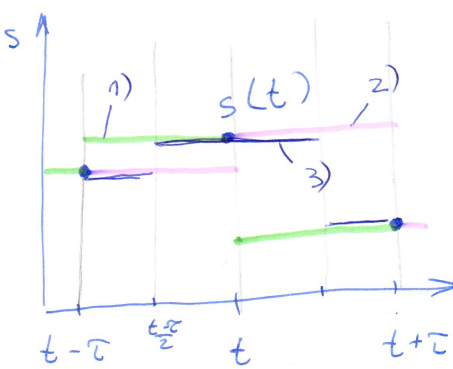
\includegraphics[width=0.4\textwidth]{resample1.png}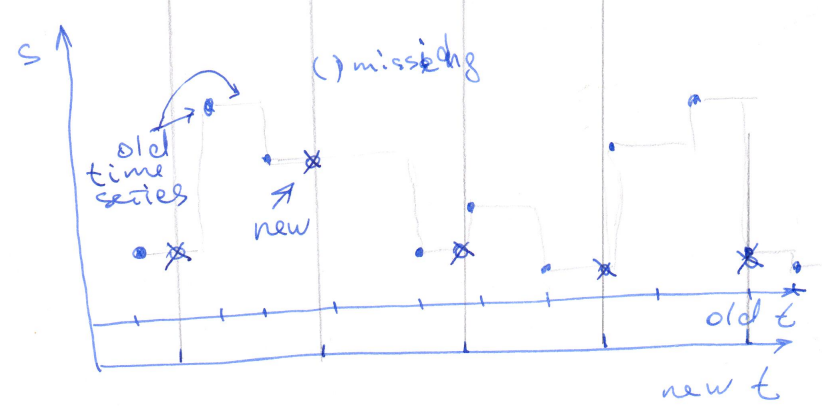
\includegraphics[width=0.5\textwidth]{resample2.png}


\end{frame}
%-----------------------------------------------------------------------------------------------------

\end{document} 